%*********************************************************************************
% 
% Paper Title Here 
%
%

\documentclass[pageno]{jpaper}

%***********************************************************************************
%
% Packages
%

\usepackage[normalem]{ulem}

\usepackage{graphicx}
%\usepackage{subfigure}
%\usepackage{psfrag}
%\usepackage{fullpage}

\usepackage{flushend}

\usepackage{tsgcomments}

%***********************************************************************************
%
% MACROS start
%

%myfigure label content caption
\newcommand{\myfigurewide}[3]
{\begin{figure*}[hbtp]\begin{center}#2\caption{#3}\label{#1}\end{center}\end{figure*}}

%mygraphfigure label size content caption
\newcommand{\mygraphfigurewide}[4]{\myfigurewide{#1}{\includegraphics[#2]{#3}}{#4}}

%myfigure label content caption
\newcommand{\myfigure}[3]
{\begin{figure}[hbt]\begin{center}#2\caption{#3}\label{#1}\end{center}\end{figure}}

%mygraphfigure label size content caption
\newcommand{\mygraphfigure}[4]{\myfigure{#1}{\includegraphics[#2]{#3}}{#4}}

%mygraphsubfigure label size content caption
\newcommand{\mygraphsubfigure}[4]
{\subfigure[#4]{\hspace{0.5cm}\includegraphics[#2]{#3}\label{#1}\hspace{0.5cm}}}

\newtheorem{theorem}{Theorem} % SMALL
\newtheorem{definition}{Definition} % SMALL
\newtheorem{problem}{Problem} % SMALL
\newtheorem{lemma}{Lemma} % SMALL

%***********************************************************************************
%
% Anonymization Macros
%

% Usage : \ifanonymized{anonymized}{notanonymized}

% Uncomment one of the following

\newcommand{\ifanonymized}[2]{#1} % Anonymized
%\newcommand{\ifanonymized}[2]{#2} % Not Anonymized
                                   
%***********************************************************************************
%
% MACROS end
%

\begin{document}  

% Note : You should only include files here. The actual content is in
% the included files.

\title{
%Dataflow-Guided Filtering for Efficient and Adjustable Run-Time Monitoring
%Efficient and Adjustable Run-Time Monitoring Using Dataflow-Guided Filtering
Run-Time Monitoring with Adjustable Overheads \\Using Dataflow-Guided Filtering
}

\ifanonymized{\author{Anonymized}}
{\author{Daniel Lo, Tao Chen, Mohamed Ismail, and G. Edward Suh}}

\date{}
\maketitle

\thispagestyle{empty}

\begin{abstract}

Recent studies have proposed various parallel run-time monitoring techniques to
improve the reliability, security, and debugging capabilities of computer
systems. However, these run-time monitors can introduce large performance and energy
overheads, especially for flexible systems that support a range of monitors.
%Traditionally, these overheads have been an
%all-or-nothing cost; monitoring cannot be used if the overheads are considered
%too large.  
In this paper, we introduce a hardware dataflow tracking engine that enables
adjustable overheads through partial monitoring. This allows a trade-off to be
made between monitoring coverage and overhead. This dataflow engine
can also be extended to filter out monitoring operations associated with null
metadata in order to reduce overheads.
% In this paper, we introduce a hardware dataflow tracking engine that can be
% used to filter out unnecessary monitoring and enable adjustable partial monitoring.
% The dataflow engine can identify events with null metadata so that they can
% be filtered out. To further reduce the overhead of monitoring, we propose
% to enable a trade-off between monitoring coverage and overhead by dropping certain
% monitoring operations. For this partial monitoring, the dataflow engine is used
% to track dropped monitoring flows so that false positives can be avoided.
Given this architecture, we investigate how the dropping decisions should be
made for partial monitoring and show that there exist interesting policy
decisions depending on the target application of partial monitoring.
Our experimental results show that overheads can be reduced significantly 
by trading off coverage. For example, for monitoring techniques with average
overheads of 3-4x, the proposed architecture is able to reduce slowdowns to
1.5x while still achieving 43-82\% average coverage. 

\end{abstract}

\section{Introduction}
\label{sec:intro}

% Parallel run-time useful
Run-time monitoring techniques have been shown to be useful for improving the
reliability, security, and debugging capabilities of computer systems. For
example, Hardbound is a hardware-assisted technique to detect out-of-bound
memory accesses, which can cause undesired behavior or create a security
vulnerability if uncaught \cite{hardbound-asplos08}.  Intel has
recently announced plans to support buffer overflow protection similar to
Hardbound in future architectures \cite{intel-mpx}. Similarly, run-time
monitoring can enable many other new security, reliability, and debugging
capabilities such as fine-grained memory protection \cite{mondrian-asplos02},
information flow tracking \cite{dift-asplos04, testudo-micro08}, hardware error
detection \cite{argus-micro07}, data-race detection \cite{radish-isca12,
cord-hpca06}, etc. 

% Programmable hardware monitors
These run-time monitors introduce performance, power, and energy overheads.
Implementing run-time monitoring in software using binary instrumentation or
other similar methods introduces high overheads. For example,
dynamic information flow tracking (DIFT) implemented in software suffers a 3.6x
slowdown \cite{lift-micro06}. Implementing monitors in hardware greatly decreases
the performance impact by performing monitoring in parallel to a program's
execution. A dedicated hardware implementation of DIFT reduces performance
overheads to just 1.1\% \cite{dift-asplos04}. However, fixed hardware loses
the programmability of software, and cannot be updated or changed.

% Recent studies proposed programmable parallel hardware as a way to achieve both
% the performance advantages of hardware and the flexibility of software
% \cite{lba-isca08, flexcore-micro10, harmoni-dsn12}.  While more
% efficient than software, these programmable hardware monitors can still show
% significant performance overheads.  For example,
% Figure~\ref{fig:intro.full_mon} shows the execution time for three monitoring
% techniques normalized to the execution time with no monitoring for an
% FPGA-based parallel monitor. The program being monitored is run on an in-order
% embedded core running at 500 MHz while the FPGA-based monitor runs at 250 MHz.
% We can see that, depending on the monitoring scheme, overheads can easily be
% several tens of percent.  A faster or more complex (e.g., superscalar or
% out-of-order) core is expected to show even more significant overheads.

% % Run-time monitoring overview
% \begin{figure}
%   \begin{center}
%     \vspace{-0.2in}
%     \includegraphics[width=\columnwidth]{figs/full_mon.pdf}
%     \vspace{-0.5in}
%     \caption{Performance overheads of FPGA-based monitors.}
%     \vspace{-0.2in}
%     \label{fig:intro.full_mon} 
%   \end{center}
% \end{figure}

In this paper, we present an architecture that combines hardware-based dynamic
information flow tracking with a software-based monitor in order to reduce the
overheads of monitoring. By using the DIFT engine to filter out events that do
not correspond to valid metadata, we can greatly reduce the amount of
monitoring that must be handled by the monitor. For example, for an array
bounds check, we are able to filter out instruction that do not correspond to
pointer data. Since the monitor is implemented in software, the system allows a
large range of monitors to be implemented and even updated or changed at
run-time. 

With this filtering, we see overheads of XX\% - XX\% on average for
uninitialized memory check, array bounds check, and multi-bit dynamic
information flow tracking. Although full monitoring coverage is always desired,
if these overheads are considered too high by the designer or user then
monitoring must be disabled.
% % Current schemes are all-or-nothing: suffer full performance impact for full
% % coverage.
% Traditionally, these overheads have been an all-or-nothing cost. If the
% designer finds that the overheads exceed their desired budget, then monitoring
% cannot be enabled.  In this paper, we present an architecture that enables a
% trade-off between the overheads and the coverage of a monitoring technique by
% dynamically adjusting the number of monitoring operations.  This system allows
% monitoring to still be performed even when the overhead budget is not
% sufficient for full monitoring.
% Use cases
Trading off coverage for
reduced overheads can still be very useful. For example, this adjustable
monitoring enables a level of protection even for systems where the full
monitoring overheads are too high.  This is especially true for energy- or
power-constrained systems or soft real-time systems where the monitoring
overhead should not exceed energy/power limits or real-time deadlines. 
Additionally, adjustable monitoring can be used for debugging purposes
especially in the context of sampling-based or cooperative debugging techniques
which expect low coverage per run but use a large number of runs and users to
collect debugging information~\cite{liblit-pldi05,
chilimbi-asplos04, greathouse-cgo11}. 

Thus, we develop an architecture that enables a
trade-off between the overheads and the coverage of a monitoring technique by
dynamically adjusting the number of monitoring operations. By extending the
hardware DIFT engine to track 2-bits of information, we are able to use it for
filtering empty metadata as well as tracking dropped monitoring flows in order
to prevent false positives. We introduce three policies of where dropping
decisions are made and show the trade-off space achieved between accuracy of
overhead matching and coverage achieved.

% %Invalidation in order to prevent false positives.
% In order to adjust monitoring overheads, a system must be able to drop a
% portion of the monitoring operations. Unfortunately, however, simply skipping
% monitoring operations can lead to false positives (false alarms) due to stale
% metadata.  One possible solution is to rewrite individual monitors to create
% ``drop-enabled'' versions.  However, such monitor-specific customizations are
% difficult and time consuming.  Instead, after analyzing a range of monitoring
% techniques, we found that by adding a 1-bit ``invalid'' flag to the bookkeeping
% metadata managed by the monitor, we were able to create a general mechanism to
% handle false positives across a broad range of monitoring techniques.  The
% result is that we have designed a hardware module that sits between a
% processing core and a programmable monitor, and allows adjustable overheads.
% This hardware module can be applied to a range of monitoring techniques and
% requires no modifications to the monitor.

% Evaluation
In order to evaluate our approach, we applied it to 3 different monitoring
techniques. These monitoring techniques vary in what events they monitor, the
size and semantics of their metadata, and the operations performed on metadata.
Our experiments show that with 10\% overheads, we can still provide 49-90\% of
coverage on average depending on the monitoring technique. By increasing the
overhead budget, the coverage rate can be increased. Our architecture is able
to closely meet the specified budgets. For all but one benchmark, the overheads
seen were within 2\% of the target overhead. Our results show that X policy is
able to achieve very close overhead matching (within X\% on average) with an
average coverage of X\%. On the other hand, by using Y policy, the overhead
matching is not as high (within Y\% on average) but average coverage increases
to (Y\%).

% Section summary
This paper is organized as follows. Section~\ref{sec:monitoring} presents the
parallel run-time monitoring model that this paper assumes.
Section~\ref{sec:filter} presents our architecture that use hardware-based DIFT
in order to reduce monitoring overheads. In Section~\ref{sec:drop} we present
how the DIFT engine can be extended to enable adjustable overheads.
Section~\ref{sec:extensions} covers example implementations of three monitoring
schemes. Section~\ref{sec:evaluation} presents our evaluation methodology and
results. Finally, we discuss related work in Section~\ref{sec:related} and
conclude in Section~\ref{sec:conclusion}.


\section{Adjustable Run-Time Monitoring}
\label{sec:monitoring}

% Previous work overheads
\begin{table*}[t]
  \begin{center}
    \vspace{-0.0in}
    \begin{footnotesize}
    %\begin{tabular}{|l|p{2in}|r|r|}
\begin{tabular}{|l|l|l|r|}

\hline
{\bf Name} & {\bf Type} & {\bf Monitoring scheme and flexibility} & {\bf Slowdown (avg./worst)} \\ \hline\hline

DIFT \cite{dift-asplos04} & Custom HW & DIFT only & 1.1\% / 23\% \\ \hline
FlexiTaint \cite{flexitaint-hpca08} & Custom HW & DIFT w/ programmable policies & 1.1\%-3.7\% / 8.7\% \\ \hline
Hardbound \cite{hardbound-asplos08} & Custom HW & Array bounds checks only & 5\%-9\% / 22\% \\ \hline
Harmoni \cite{harmoni-dsn12} & Custom HW & Tag-based monitors & 1\%-10\% / 20\% \\ \hline\hline

FlexCore \cite{flexcore-micro10} & Dedicated FPGA & Instruction-trace monitoring & 1.05x-1.44x / 1.84x \\ \hline
FADE \cite{FIXME} & Core+Custom HW & Instruction-trace monitoring (effective when HW filters work) & \\ \hline
LBA-accelerated \cite{lba-isca08} & Multi-core+Custom HW & Instruction-trace monitoring (effective when accelerators work) & 1.02x-3.27x / 5x \\ \hline
LBA \cite{lba-asid06} & Multi-core+Custom HW & Instruction trace monitoring & 3.23x-7.80x / 11x \\ \hline \hline

Multi-core DIFT \cite{nagarajan-interact08} & SW (multithreaded) & DIFT (compiled for each application) & 1.48x / 2.2x \\ \hline

LIFT \cite{lift-micro06} & SW (DBI) & DIFT (fully flexible) & 3.6x / 7.9x \\ \hline
Purfiy \cite{purify-usenix92} & SW (DBI) & Memory leak checks (fully flexible) & 2.3x / 5.5x \\ \hline
TaintCheck \cite{taintcheck-05} & SW (DBI) & DIFT (fully flexible) & 10x / 27x \\ \hline


\end{tabular}

    \end{footnotesize}
    \caption{Trade-off between performance overhead and flexibility/complexity of run-time monitoring systems.}
    \vspace{-0.2in}
    \label{tab:monitoring.previous_overheads}
  \end{center}
\end{table*}

\subsection{Overhead of Run-Time Monitoring}

There have been a number of proposals for run-time monitoring systems exploring various
design points. % in the trade-off space between efficiency and flexibility.
Table~\ref{tab:monitoring.previous_overheads} summarizes some of representative designs
and their reported performance overhead. The previous studies clearly show that there
exist trade-offs among efficiency, flexibility, and hardware costs. 
For example, a run-time monitoring scheme can often be realized with fairly low
performance overhead (less than 20\%) if implemented with custom hardware that is
designed only for one monitor or a narrow set of monitors. However, the custom
hardware monitors cannot be modified or updated, and require dedicated silicon area. 
On the other hand, flexible systems that support a wide range of monitors lead 
to noticeable performance overhead, often too high for wide deployment in practice.
Software-only implementations \cite{nagarajan-interact08, lift-micro06,
purify-usenix92, taintcheck-ndsss05} or multi-core monitors with minimal
hardware changes \cite{lba-asid06} are reported to have severalfold slowdowns.
On-chip FPGA monitors \cite{flexcore-micro10} and cores with monitoring accelerators
\cite{lba-isca08, fade-hpca14} can reduce overhead significantly, but still show
slowdowns of several tens of percents in some cases.
In today's monitoring systems, the overhead is also unpredictable because they
depend heavily on the characteristics of applications and monitoring operations.
In summary, users currently need to either pay noticeable overhead or the cost of custom
hardware in order to use fine-grained run-time monitoring in deployed systems.

\subsection{Partial Monitoring for Adjustable Overhead}

In this paper, we aim to develop a general framework that enables monitoring
overhead to be dynamically adjusted by dropping a portion of monitoring 
operations if necessary. In essence, this framework adds a new dimension to
the monitor design space by allowing coverage or accuracy to be traded off
for lower overhead. For example, the capability to adjust overhead allows users
to use monitoring with partial coverage in order to reduce performance
or energy overhead. Alternatively, partial monitoring allows designers to use
less expensive hardware for a given performance overhead budget.
%simple hardware such as a
%multi-core without elaborate acceleration features to provide partial monitoring
%with the performance overhead that is comparable to custom hardware.

In this framework, a user specifies how much monitoring should be done in a form of
a target 
overhead budget, a target coverage, a percentage of monitoring operations to be performed, etc.
Then, the framework dynamically drops a portion of monitoring operations to match
the target. In particular, this paper focuses on matching a performance overhead target
while maximizing the coverage. Given that the overhead of custom hardware monitors can
already be quite low, the focus is on enabling the trade-off in {\em general-purpose} 
monitoring systems that support a wide range of monitors.
We also consider the target overhead as a soft constraint and do not aim to
provide a strict worst-case guarantee.

\subsection{Applications and Metrics}

While it is ideal if run-time monitoring can be performed in full, we believe that
the capability to trade-off coverage/accuracy for lower performance/hardware overhead
will be useful in many application scenarios where full monitoring is not a viable option.
Here, we briefly discuss example applications of partial monitoring and the metrics
that are important in each case.

{\bf Cooperative testing, debugging, and protection:}
Recently studies \cite{liblit-pldi05, chilimbi-asplos04, greathouse-cgo11, testudo-micro08} have shown that software testing, debugging,
or attack detection may be done in a cooperative fashion across
a large number of systems. In this case, each system is only willing to pay very low
overhead, say a few percents, and only performs a small subset of checks. 
A high coverage is achieved by having different systems check different parts of a program.
The partial monitoring framework allows high-overhead monitoring to be used in a
cooperative fashion. 
The main metric that represents the effectiveness of monitoring in this case is
the coverage (the percentage of checks there were performed) over multiple runs.

{\bf Monitoring of soft real-time systems:}
Soft real-time systems or interactive systems need to meet deadlines or response
time requirements. Unfortunately, the overhead of run-time monitoring is often 
unpredictable and varies significantly depending on the application and monitor
characteristics. The partial monitoring framework allows monitoring to be performed
while providing a level of guarantee on its impact on the execution time. 
In this case, it is important that the system can closely match the desired
overhead target while maximizing the effectiveness of monitoring.

{\bf Partial protection for low overhead:}
Even without real-time constraints, systems may have tight budgets for performance,
energy, or hardware overhead that they can tolerate for run-time monitoring. In such cases,
full monitoring cannot be enabled unless its overhead is low enough. The adjustable
monitoring allows partial protection on such systems. For example, array bounds
may be checked for a subset of memory accesses. For DIFT, a subset of information flows
may be tracked for partial attack detection. In this scenario, the effectiveness of 
partial monitoring can be measured as the percentage of run-time checks that are
performed on each program run, which reflects how likely for a bug or an attack 
to be detected for a system. 

{\bf Profiling:} 
The run-time monitoring system can be used to implement various profiling tools
to collect statistics on program behaviors for performance optimizations as well
as security protection. For example, a recent study showed that an instruction
mix can be used to identify malware from normal programs \cite{demme-isca13, tang-raid14}. 
In such profiling tools, the partial monitoring framework can be used to obtain
the statics on samples rather than all program events, essentially trading off
accuracy for lower overhead.

\subsection{Design Challenges}

While conceptually simple, designing a general framework to dynamically adjust monitoring
overhead introduces new challenges that need to be addressed.  
The following summarizes the main design goals and associated design challenges.

\begin{enumerate}
  \item \textbf{General:} Because we mainly target flexible run-time monitoring systems,
  which often have high overhead, the framework also needs to be general enough to be
  applicable to a wide range of monitoring scheme.

  \item \textbf{No false positive:} The framework needs to ensure that dropping a portion
  of monitoring operations does not lead to a false positive. We found that a data-flow
  that tracks invalid meta-data can serve as a general solution to this problem 
  (Section~\ref{sec:dropping}).

  \item \textbf{Intelligent dropping:} The framework needs to match the overhead budget
  while maximizing the effectiveness of monitoring. To this end, partial 
  monitoring needs to carefully choose which operations to drop and when. We address this
  problem by studying different dropping policies (Section~\ref{sec:policies}) and their
  trade-offs.

\end{enumerate}


\section{Architecture for Adjustable Monitoring}
\label{sec:dropping}

In this section, we present our hardware architecture that enables partial
monitoring for adjustable overheads. Section~\ref{sec:dropping.baseline} first
describes our baseline model for run-time monitoring while the rest of the
section describes our design.

\subsection{Baseline Architecture}
\label{sec:dropping.baseline}

% Run-time monitoring overview
\begin{figure}
  \begin{center}
    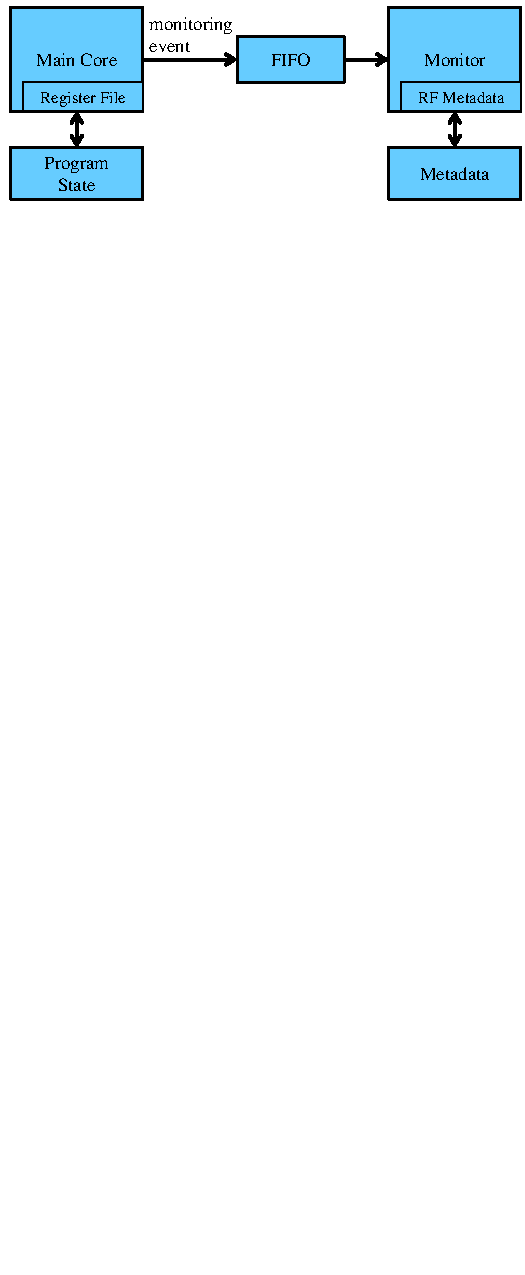
\includegraphics[width=\columnwidth]{figs/monitoring_architecture.pdf}
    \vspace{-0.2in}
    \caption{Overview of run-time monitoring architecture.}
    \label{fig:dropping.overview} 
    \vspace{-0.1in}
  \end{center}
\end{figure}

Figure~\ref{fig:dropping.overview} shows an overview of the run-time monitoring
model that is assumed in this paper.  The \emph{main program} is a computation
task that performs the original function of the system and is run on the
\emph{main core}.  On certain events during the main program, such as the
execution of certain types of instructions, the \emph{monitor} performs a
series of \emph{monitoring operations}. The monitor operates in parallel to the
main core. Events that trigger monitoring are referred to as \emph{monitoring events}. Depending
on the type of monitoring event, different monitoring operations are
executed. Information about monitoring events is sent to the monitor and
buffered in a FIFO structure to decouple the
running of the main core and the monitor. If the FIFO is full, then the main
core is forced to stall on a monitoring event until a FIFO entry becomes
available. These stalls are a major source of
overhead because the monitor may take several cycles to process a single event
from the main core. 
Monitors typically maintain metadata corresponding to each memory location
({\tt mem\_metadata[addr]}) and register ({\tt rf\_metadata[reg\_id]}) of the
main core.
If the monitor
detects an inconsistent or undesired behavior in the monitoring events, then
an error is detected. 

There are many possible monitoring schemes that can be implemented on this type
of fine-grained parallel monitoring architecture such as memory protection
\cite{mondrian-asplos02}, information flow tracking \cite{dift-asplos04,
testudo-micro08}, soft error detection \cite{argus-micro07}, data-race
detection \cite{cord-hpca06, eraser-tocs97, literace-pldi09, pacer-pldi10}, etc.  For example, an array bounds check (BC)
\cite{hardbound-asplos08} can be implemented in order to detect
when software attempts to read or write to a memory location outside of an
array's bounds. This can be done by associating metadata with array pointers that 
indicates the array's base (start) and bound (end) addresses. On loads or stores with the
array
pointer, the monitor checks that the memory address accessed is within the base and
bound addresses. In addition, this base and bound metadata
is propagated on ALU and memory instructions to track the corresponding array pointers.
% One example is an uninitialized memory check (UMC) where monitoring is used to
% detect when software attempts to read from a memory location that was not
% previously initialized. This can be done by forwarding each load and store
% instruction from the main core to the monitor. For every memory location, the
% monitor keeps one bit of metadata. On a store to a memory location, the monitor
% marks the corresponding metadata bit to indicate that the memory location has
% been initialized. On a load, the monitor checks that the corresponding metadata
% bit has been previously marked as initialized.

% There are multiple options for implementing programmable parallel monitors. For
% example, the Log-Based Architecture \cite{lba-isca08} uses processor cores in a
% multi-core system as monitors. The FlexCore architecture
% \cite{flexcore-micro10} instead uses an FPGA-fabric to implement the
% monitor. 
% 
% The approach we describe in this paper applies to any of these
% parallel monitors. However, for experiments, we model an FPGA-based monitor
% similar to FlexCore.  The on-chip FPGA fabric is used to implement the
% ``Monitor'' block in Figure~\ref{fig:arch.overview} while the FIFO from the
% main core and metadata cache are implemented as ASICs.

% Example monitor
\begin{figure*}
  \begin{center}
    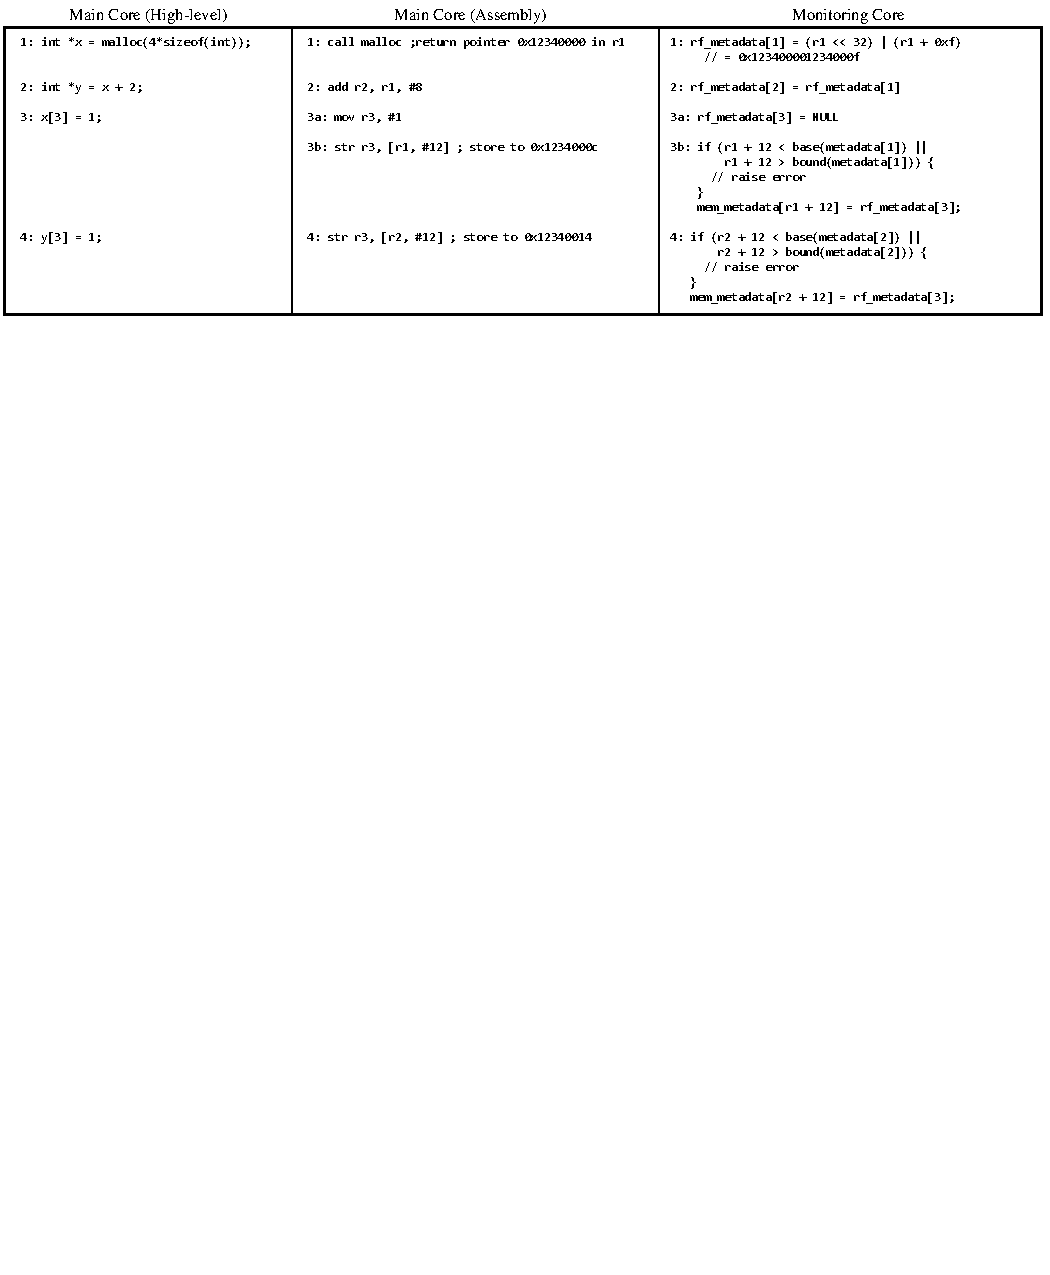
\includegraphics[]{figs/example_full.pdf}
    \caption{Example of array bounds check monitor.}
    \label{fig:dropping.example_full}
    \vspace{-0.1in}
  \end{center}
\end{figure*} 

Figure~\ref{fig:dropping.example_full} shows an example pseudo-code segment,
its assembly level instructions, and the corresponding monitoring operations
for an array bounds check monitor. 
First, an array {\tt x} is allocated using {\tt malloc} (line 1). 
As {\tt malloc} returns the array's address in a register, the monitor
associates base and bounds metadata with the corresponding register. 
Next, pointer {\tt y} is set to point to the middle of array {\tt x} (line 2). 
At the assembly level, a register {\tt r2} is set to array {\tt x}'s address plus an offset.
The monitor propagates the metadata of the original pointer in {\tt r1} to the
metadata of {\tt r2}. This is to ensure that pointer {\tt y} is not used to exceed the array's bounds.
Line 3a shows setting register {\tt r3} to a constant value of 1.
When this happens,
{\tt r3}'s metadata is reset to NULL in case it previously stored a
pointer. 
Finally, the value of {\tt r3} is written to memory using both pointers {\tt x} and {\tt y}.
In both cases, the monitor checks whether the store address is within the bounds of the register metadata. In the first case (line 3b), {\tt x+12}
is within the original array's bounds. No error is raised and the metadata of
{\tt r3} is propagated to the metadata of the store address. If {\tt r3} were a
pointer, then this would allow a future instruction to load the pointer and use
it to access the corresponding array or data structure. In the second case,
{\tt y+12} (line 4) corresponds to {\tt x+20} which is not within the array's bounds and
the monitor will raise an error. 

Note that this monitoring is performed automatically and transparently with
almost no modification needed to the main program. The only modification to
the main program that is needed is to initially set metadata, such as setting
the base and bounds addresses on a {\tt malloc} call for array bounds check.
The propagation and checks of the metadata occur automatically as
instructions are forwarded.
Here, we have shown the dynamic sequence of operations executed by the monitor but
the actual static code consists of a set of instructions to be run for each
possible instruction type (load, store, etc.). Only instruction types relevant
for the particular monitoring scheme are forwarded.

% \subsection{Architecture Overview}
% 
% % Overview of full architecture
% %\begin{figure}
% %  \begin{center}
% %    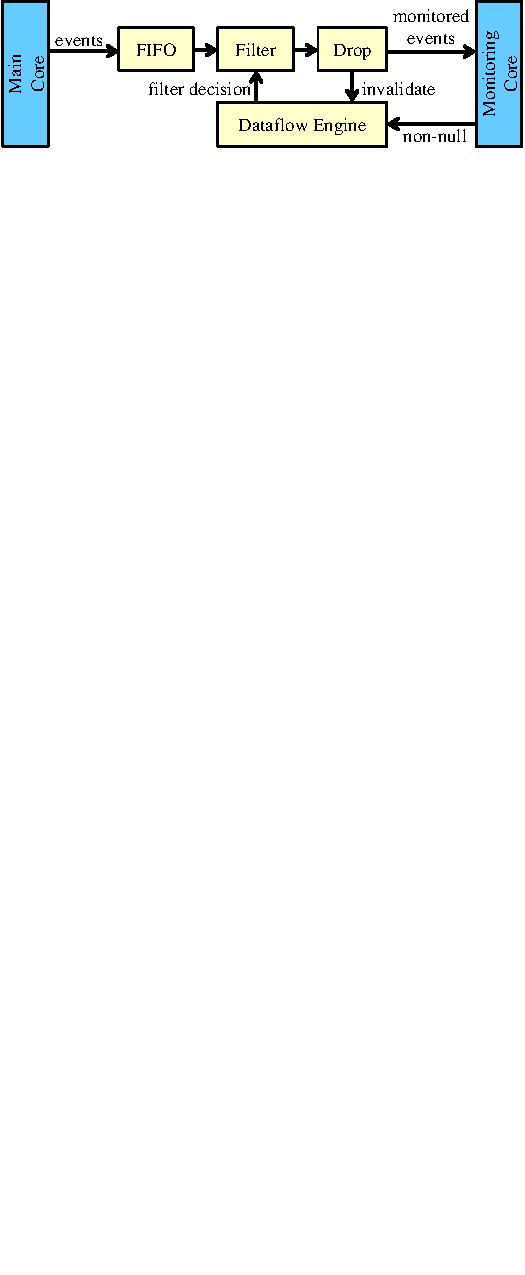
\includegraphics[width=\columnwidth]{figs/architecture_overview.pdf}
% %    \vspace{-0.2in}
% %    \caption{Block diagram of architecture for monitoring with reduced and adjustable overheads.}
% %    \label{fig:dropping.overview}
% %    \vspace{-0.1in}
% %  \end{center}
% %\end{figure}
% 
% Figure~\ref{fig:dropping.overview} shows a high-level block diagram of our
% proposed architecture for enabling partial monitoring. The basic idea is to
% insert hardware between the main core and the monitoring core to transparently
% drop monitoring events. 
% 
% There were three main challenges in designing this dropping hardware:
% \begin{enumerate}
%   \item \textbf{General:} The hardware needs to be applicable to a wide range of monitoring schemes.
%   \item \textbf{No false positives:} False positives should never occur as a result of dropping.
%   \item \textbf{Intelligent dropping:} The hardware needs to maximize the amount of useful monitoring done while staying within the overhead budget.
% \end{enumerate}
% 
% In order to reduce overheads, the ``Drop'' module decides when monitoring event
% should be skipped.  This decision of when to drop and which monitoring events
% to dropped is discussed in more detail in Section~\ref{sec:policies}.
% 
% When an event is dropped, metadata needs to be invalidated in order to prevent
% false positives. This is done using a hardware dataflow engine.
% Sections~\ref{sec:dropping.false_neg_pos} and
% \ref{sec:dropping.prevent_false_pos} discuss these false positive issues and
% the dataflow engine in detail. 
% 
% In addition, we can use the dataflow engine to filter out monitoring operations
% that would be operating on invalid metadata. This maximizes the useful
% monitoring that is done by the monitoring core.
% Section~\ref{sec:dropping.filter} talks about how this is done using
% information from the dataflow engine.

\subsection{Effects of Dropping Monitoring}
\label{sec:dropping.false_neg_pos}

Our goal is to drop some monitoring operations in order to reduce the overheads
of run-time monitoring. This dropping can affect the functionality of the
monitoring schemes. There are three possible outcomes for dropping a
monitoring operation. The first is that there is no difference in operation
from the original execution. For example, if we drop line 3b from our array
bounds check example (Figure~\ref{fig:dropping.example_full}), then the
check on accessing {\tt x+12} is skipped. However, this is a valid access and so
skipping the check does not change anything.

On the other hand, if the monitoring for accessing memory location {\tt y+12} on
line 4 is skipped, then
a false negative occurs. Originally, the monitor would catch this access as an
out-of-bounds access and raise an error. However, if the monitoring operation
for this is dropped, then the error is not detected. This reflects the trade-off that
we make in order to reduce overheads. Instead of either 100\% coverage
with all the associated overheads or no coverage and no overheads, we 
enable middle points of partial coverage with some fraction of the full
overheads.

The final possible outcome of dropping a monitoring operation is a false positive. 
For example, suppose the monitoring for
line 1 is dropped, causing the bound information for pointer {\tt x} to never
be set. The result is that when the access using {\tt x} is checked on line 3b,
an error will be raised. This creates a false positive where an error is
incorrectly raised. Although false negatives are part of the trade-off we make
to reduce overheads, we need to prevent false positives.

\subsection{Invalidation for Preventing False Positives}
\label{sec:dropping.prevent_false_pos}

% In analyzing various monitoring schemes, we found that monitoring operations
% are primarily of two types: \emph{checks} and \emph{metadata updates}. Monitors
% \emph{check} certain properties to ensure correct main program execution (lines
% 3b-4 of Figure~\ref{fig:monitoring.example_full}) and they \emph{update} metadata
% for bookkeeping (lines 1-3a of Figure~\ref{fig:monitoring.example_full}). Skipping
% a check operation can only cause false negatives and will never cause a false
% positive (see Figure~\ref{fig:dropping.example_no_error} and
% Figure~\ref{fig:dropping.example_false_negative}). Therefore, we may simply
% skip a check operation. Skipping an update operation can cause false
% negatives but may also cause false positives (see
% Figure~\ref{fig:dropping.example_false_positive}). 

% Example with invalidation
\begin{figure*}
  \begin{center}
    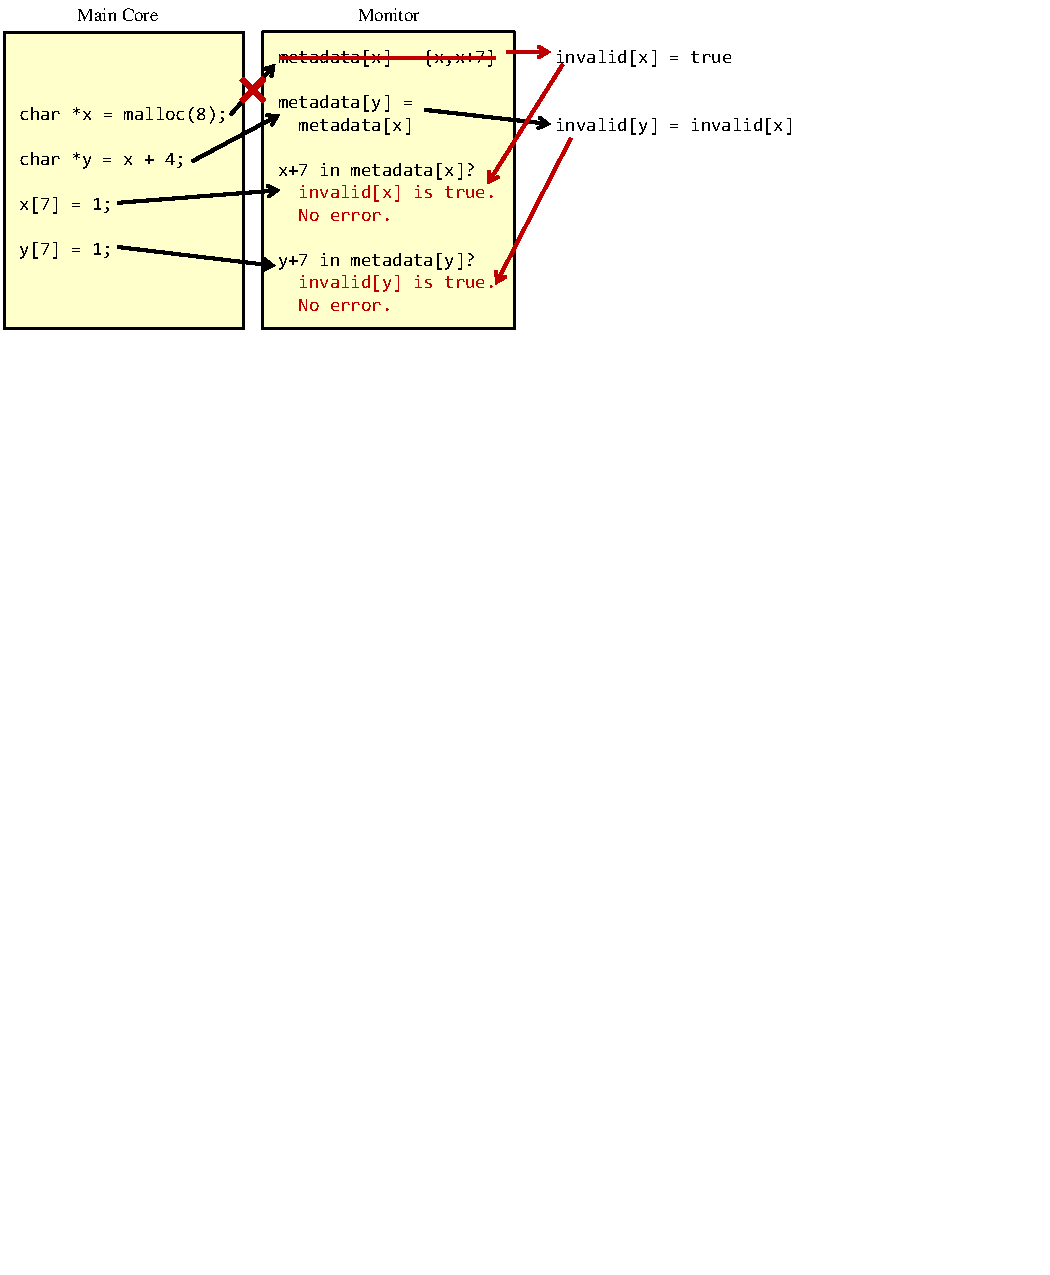
\includegraphics[]{figs/example_invalid.pdf}
    \caption{Example of using invalidation information to prevent false positives.}
    \label{fig:dropping.example_invalid}
    \vspace{-0.1in}
  \end{center}
\end{figure*}

The key cause of false positives is dropping monitoring operations that update
metadata. Dropping monitoring operations that check for an error (such as the check
for line 4 in Figure~\ref{fig:dropping.example_full}) can only cause
false negatives and will never cause false positives. On the other hand,
skipping monitoring operations that update metadata can lead to false positives
and false negatives.
Essentially, when an update operation is skipped, we can no longer trust the
corresponding metadata. Thus, our general approach for preventing false
positives is to associate a 1-bit flag with each metadata in order to mark these
metadata as valid or
invalid. Furthermore, this invalidation information is propagated in the same
way that metadata is. Figure~\ref{fig:dropping.example_invalid}
shows an example of associating invalidation flags with metadata. Suppose that the monitoring for
line 1 is dropped in order to meet the overhead target. When a monitoring event is dropped, metadata that would have
been updated is marked as invalid. In this case, instead of the normal
operation of marking {\tt rf\_invalid[1]} as {\tt false}, it is instead
marked as {\tt
true}. Thus, when line 3 is reached, the monitoring event is dropped
since {\tt rf\_invalid[1]} is marked as true. Note that in this case, line 2
also propagates this invalidation flag to {\tt rf\_invalid[2]} and causes the check
performed on line 4 to also be dropped. This is necessary because an error
would have been raised even if the access on line 4 was within bounds.

\subsection{Dataflow Engine for Preventing False Positives}
\label{sec:dropping.arch}

% Dataflow engine high-level
\begin{figure}
  \begin{center}
    \vspace{-0.1in}
    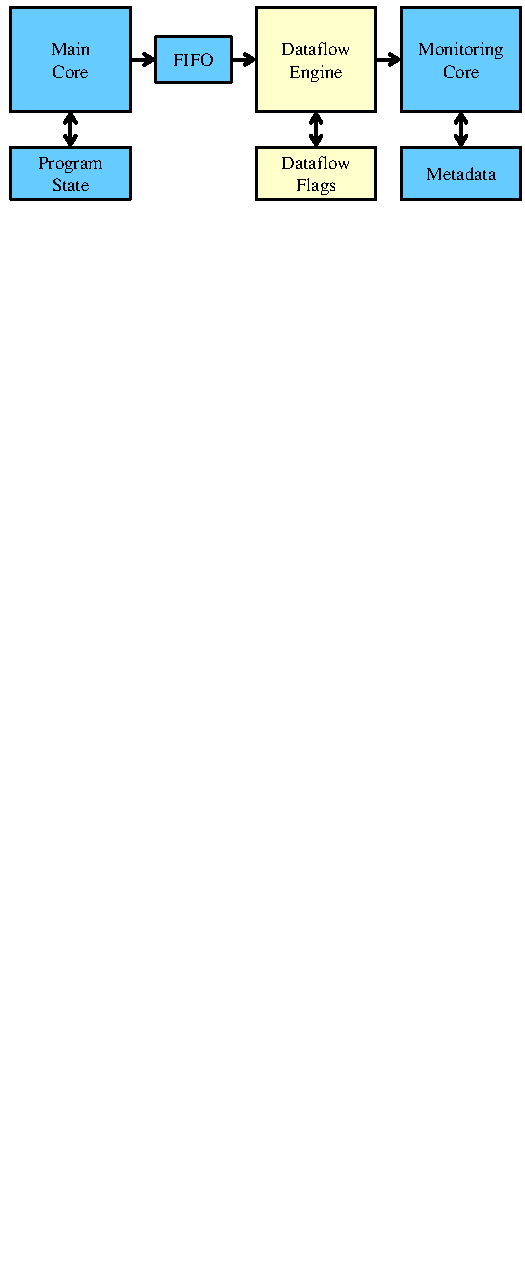
\includegraphics[width=\columnwidth]{figs/dataflow_overview.pdf}
    \vspace{-0.2in}
    \caption{Hardware support for dropping.}
    \label{fig:dropping.dataflow_overview}
    \vspace{-0.2in}
  \end{center}
\end{figure}

Although the functionality of dropping and invalidation could be implemented on
the monitor, this is unlikely to be much faster than performing the full monitoring
operations.
Instead, in order to efficiently support dropping monitoring events and to prevent false
positives, we propose to insert a hardware module between the main core and
monitor (see Figure~\ref{fig:dropping.dataflow_overview}). 
This module handles the invalidation operations shown in the middle column of
Figure~\ref{fig:dropping.example_invalid}.
There are two operations that are done for handling invalidation information:

\begin{enumerate}
  \item Propagate invalidation flags, following the dataflow of metadata.
  \item Filter out monitoring operations based on invalidation flags.
\end{enumerate}

% Detailed architecture of dataflow engine
\begin{figure*}
  \begin{center}
    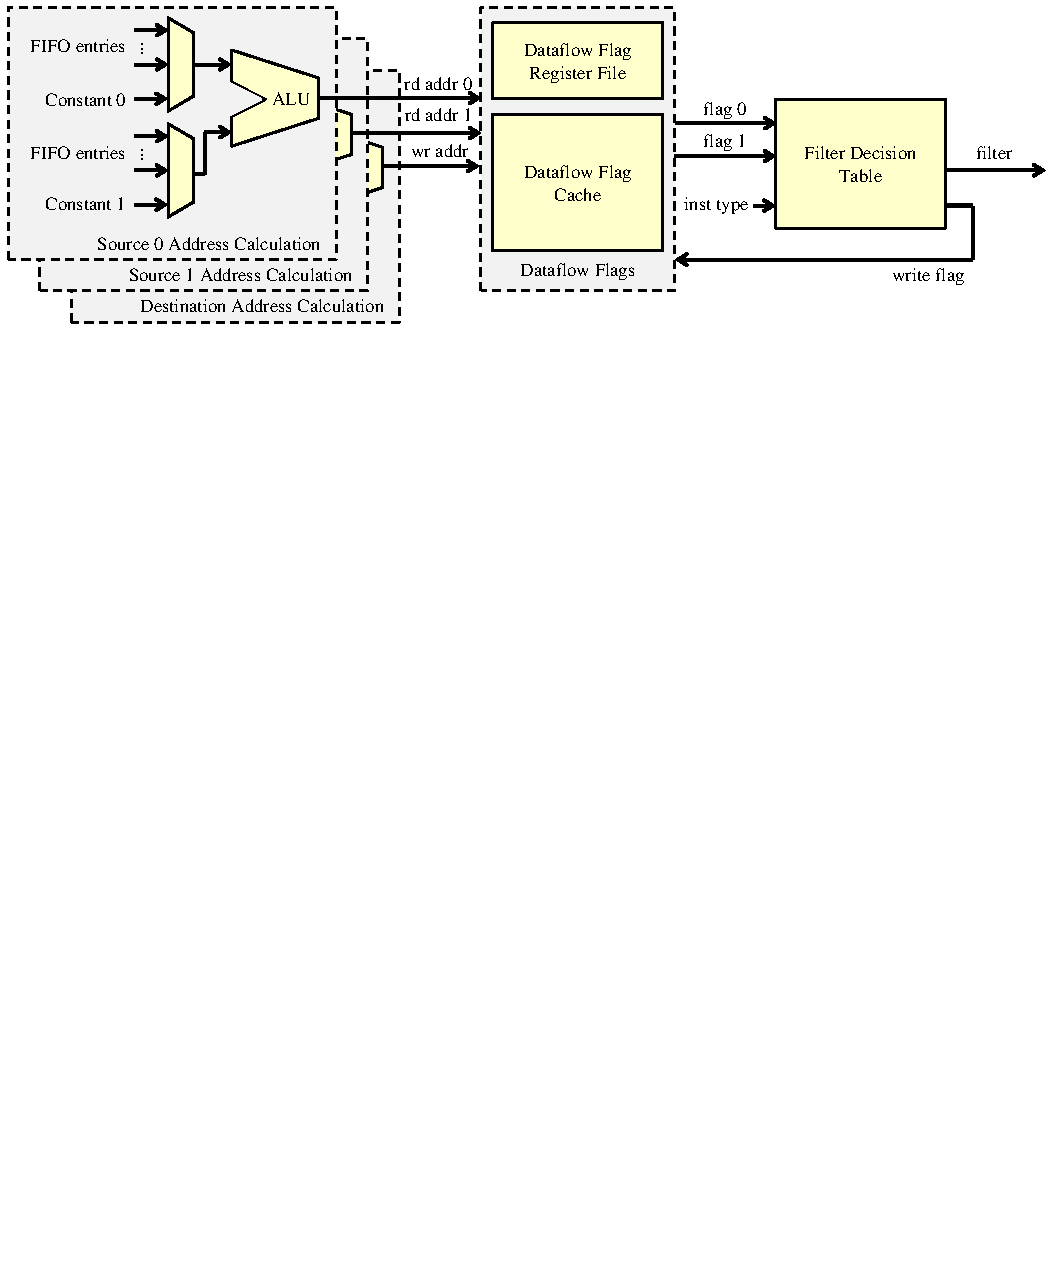
\includegraphics[]{figs/dataflow_architecture.pdf}
    \vspace{-0.1in}
    \caption{Hardware architecture of the dataflow engine.}
    \label{fig:dropping.dataflow} 
    \vspace{-0.1in}
  \end{center}
\end{figure*}

Thus, the hardware acts effectively as a dataflow tracking engine in order to
track a 1-bit invalidation flag per metadata. Figure~\ref{fig:dropping.dataflow} shows a detailed block
diagram of this hardware module. The dataflow engine uses two address
calculation units to read in up to two invalidation flags. These source invalidation flags
are used to decide whether a monitoring event should filtered. A third address
calculation unit is used to optionally specify a target to propagate the
invalidation information. The module includes a register file to store invalidation
flags corresponding to register file metadata. In addition, it uses a small
memory-backed cache to handle invalidation flags corresponding to memory metadata.

Since different monitoring operations are performed based on instruction type,
the dataflow engine is also configured based on instruction type. The source
and operation of the address generation units are set based on instruction
type. Note that the address calculation units also take information from the
monitored event as inputs. Thus, in the same way that the monitor selects
metadata based on register indices or memory address of the specific monitoring
event, the dataflow engine also reads the appropriate flags. In addition, the
filter decision table is configured based on instruction type to decide what
combination of input flags will lead to a filtered event and whether
propagation is required.

% Monitoring schemes typically keep metadata corresponding to the main core's
% register file as well as the main core's memory space. Similarly, the dataflow
% engine uses an on-chip register file to store flags for register file metadata.
% In addition, a set of flags are stored that correspond to memory metadata.
% These memory metadata flags are accessed through a cache and backed to main
% memory. All flags are initialized as valid when the system starts. 

% Address calculation and configuration
% On a monitoring event, the dataflow engine reads in up to two flags in order to
% determine whether the event can be filtered.  The flags to be read in typically correspond to the source
% operands of the monitored instruction. For example, on a load, the dataflow
% engine will typically read in the flags corresponding the memory location
% accessed.
% However, the architecture is designed such that the address of flags to be read
% is calculated dynamically and can be configured depending on the monitoring
% scheme. Specifically, there exists a configuration table that outputs a set of
% control signals depending on the instruction type of the monitoring event.
% These control signals are used to control a pair of address calculation units which each
% contain a simple ALU. The inputs to the ALU are information from the monitored
% event and a constant that is specified from the configuration table. One common
% use of this address calculation is to transform addresses from byte-addressed
% to word-addressed by right shifting the passed memory address by 2 bits.

% \subsection{Filtering Invalid Events}
% \label{sec:dropping.filter}
% 
% % Filtering decision
% The decision of whether an event can be filtered out is determined using a
% lookup table. This filter decision table is configured by the monitoring scheme
% on system initialization. The lookup table determines whether an event can be
% filtered out based on the pair of input flags read and the instruction type of
% the monitored event.
% For example, on an ALU instruction, if both of the source operand flags
% indicate that the corresponding metadata is null, then typically the instruction can be
% filtered out. Similarly, on an ALU instruction, if either of the source operand
% flags indicate that their corresponding metadata is invalid, then the
% instruction can also be filtered out. This filter decision is sent to the
% ``Filter'' block shown in Figure~\ref{fig:dropping.overview} which will simply pop
% filtered entries from the FIFO and not forward them. If an entry is not
% filtered, then this Filter block will pop the monitoring event entry from the
% FIFO and forward it along the datapath.
% 
% % Propagating flag information
% Finally, when an event is filtered out, it is necessary to propagate the flag
% information for the filtered event. In addition to the decision of whether to
% filter an event, the filter decision table also includes information about
% whether the destination flag should be written to and what value should be
% written to it. A third address calculation unit generates the write address for
% this destination flag. For example, for an ALU instruction, this will
% correspond to the destination register of the ALU instruction. If this ALU
% instruction is filtered out due to having a pair of null source operands, then
% the filter decision table will indicate that the destination register's
% corresponding flag should also be marked as null. 

% Flags are marked as invalid when a monitoring event is dropped due to
% insufficient overhead budget. Thus, whenever a monitoring event is dropped, the
% dropping hardware indicates this to the dataflow engine. The dataflow engine's
% write address is configured for the appropriate destination flag. When it
% receives an invalidation signal from the dropping hardware, the
% dataflow engine marks this destination flag as invalid.


\subsection{Filtering Null Metadata}
\label{sec:dropping.null_filtering}

% Null filtering code example
\begin{figure}
  \begin{center}
    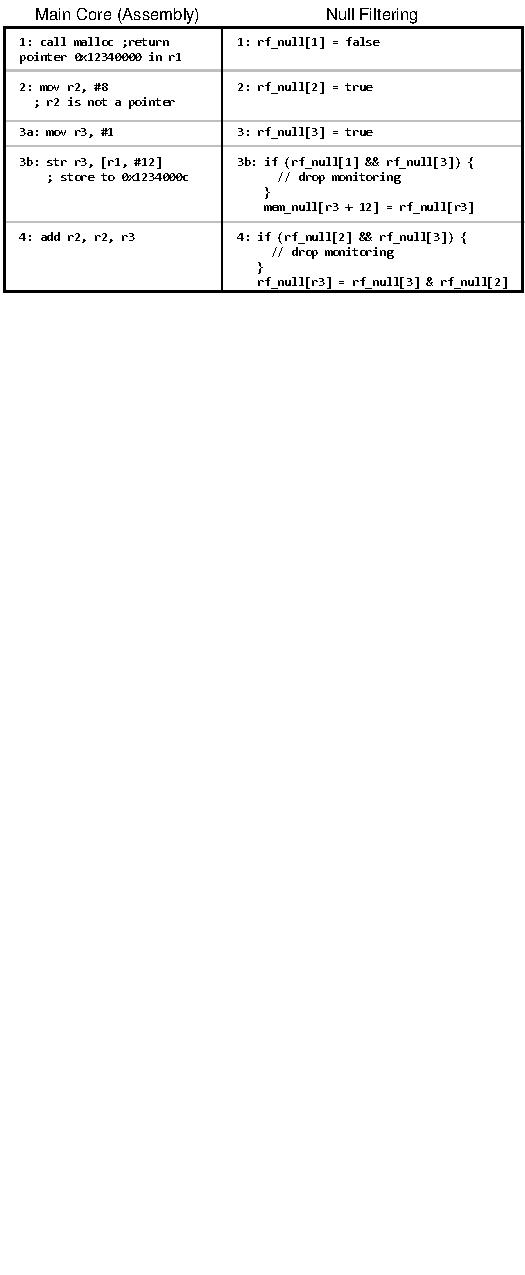
\includegraphics[width=\columnwidth]{figs/example_null_filtering.pdf}
    \vspace{-0.2in}
    \caption{Example of using information about null metadata to filter monitoring events.}
    \label{fig:dropping.example_null} 
    \vspace{-0.1in}
  \end{center}
\end{figure}

One way to reduce the number of monitoring events that must be handled by the
monitor is to filter out monitoring events that correspond to operating on null
metadata. Null metadata correspond to events that
are not relevant to the monitor. For example, Hardbound
\cite{hardbound-asplos08} filters out operations on non-pointer (i.e., no base
and bounds metadata) instructions since it is not relevant to array bounds
checking. More recently, FADE \cite{fade-hpca14} has been proposed as a general
hardware module to perform this null metadata filtering for a variety of
monitoring schemes. Our architecture is able to support this null metadata
filtering with a small modification.

Figure~\ref{fig:dropping.example_null} shows an example of how this null filtering operates.
Here, the main core's code has been slightly modified from
Figure~\ref{fig:dropping.example_full} and on line 2, {\tt r2} is no longer set as an array pointer.
Without null metadata filtering, the instruction for line 4 would be
forwarded to the monitor since the system does not know whether {\tt r2}
contains a pointer address or not. However, if we use a 1-bit flag to mark {\tt r2}
as null when it is loaded with a constant, then we can propagate this null
information and filter out monitoring for line 4.

The operations performed by null filtering are almost identical to the
operations needed for invalidation shown in
Figure~\ref{fig:dropping.example_invalid} except for a small change in the propagation policy. Instead of taking a logical OR of the
source invalidation flags to determine whether monitoring can be skipped, null
metadata filtering takes a logical AND of the source null flags.
Thus, we can easily enable this null metadata filtering on our architecture by
extending the dataflow flags to be two bits wide. One bit is used to
keep track of invalidation information while the second bit is used to keep
track of null information. All flags are initialized to null and the filter
decision table is extended with the propagation and filtering decision rules
for null metadata filtering.
The result is a single hardware design that enables both partial
monitoring and null metadata filtering.



\section{Dropping Policies}
\label{sec:policies}

In order to use partial monitoring to enable adjustable overheads, we must also
specify a policy for when and which monitoring events are dropped. In this
section, we discuss some of the options and trade-offs for dropping policies.
We split this decision into two components:
\begin{enumerate}
  \item When do we need to drop events in order to enable reduced overheads? (Section~\ref{sec:policies.when})
  \item Which events should be dropped? (Section~\ref{sec:policies.which})
\end{enumerate}

% Our goal with enabling partial monitoring is to allow for a specified overhead target or budget to be met while maximizing the amount of monitoring performed.
% This is done by dynamically dropping a portion of the monitoring operations. In this section, we discuss in detail how this dropping decision is
% made. Specifically, we first discuss how to decide when dropping should be performed 
% Section~\ref{sec:policies.slack}. Next, we investigate trade-offs created by
% selecting which events are dropped (Section~\ref{sec:policies.events}). Different policies in determining which
% events can be dropped create a trade-off between how closely the overhead
% budget is met and the monitoring coverage achieved.

\subsection{Deciding When to Drop}
\label{sec:policies.when}

% Slack
\begin{figure}
  \begin{center}
    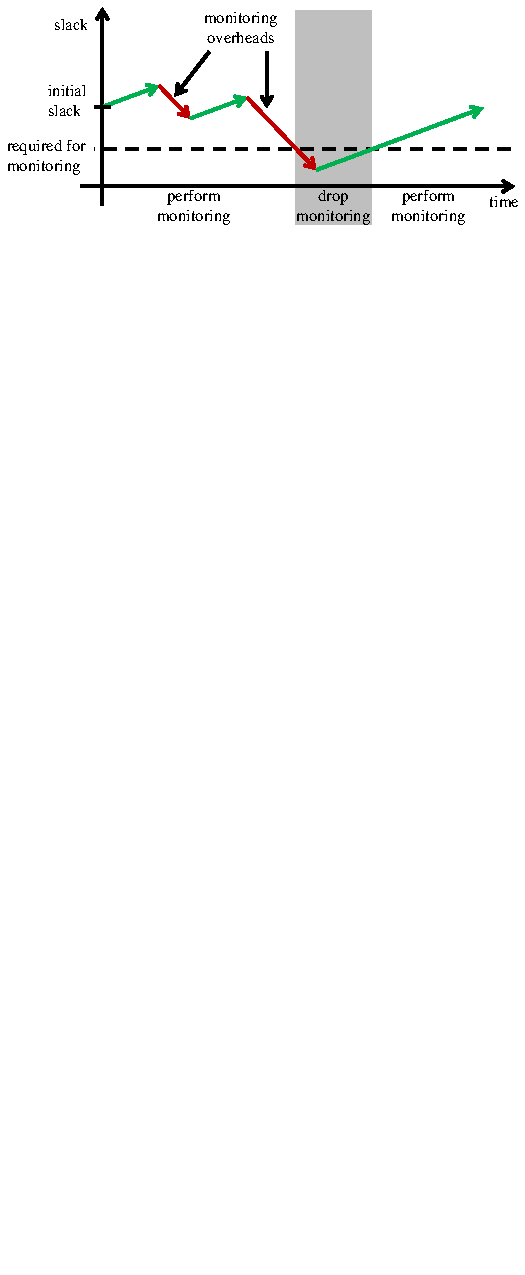
\includegraphics[width=\columnwidth]{figs/slack.pdf}
    \vspace{-0.3in}
    \caption{Slack and its effect on monitoring over time.}
    \label{fig:policies.slack}
    \vspace{-0.1in}
  \end{center}
\end{figure}

In this section, we discuss two possible ways to determine when events should be dropped.
The first possibility is to probabilistically drop events. By setting the probability of
dropping events appropriately, overheads can be reduced. This works well for
enabling partial monitoring for cooperative testing and debugging since the
randomness allows different users and runs to monitor different portions of the
program. However, using a probabilistic dropping policy can make it difficult
to meet a target overhead without prior profiling.

Alternatively, we can specify a target overhead and estimate, at run-time, the
overheads of monitoring in order to decide whether dropping is needed.
The overhead budget is specified as a percentage of the main program's execution
cycles without monitoring. We define \emph{slack} as the number of cycles of
monitoring overhead that can be incurred while staying within the budget
target. Slack is essentially the difference between the actual overheads seen
and the budget specified. Slack is generated as the main program runs and consumed as monitoring overheads occur.  For
example, if no monitoring overheads occur during 1000 cycles of the main
program's execution and the designer sets a 20\% overhead target, then the
slack that is built up during this period is 200 cycles. If the main core is
then stalled for 50 cycles due to monitoring, then the remaining slack is 150
cycles. 
In addition to this accumulated slack, a small amount of initial slack
can be given in order for monitoring to be performed at the start of a program.
Figure~\ref{fig:policies.slack} shows an example of how slack can change over time.
In this slack-based policy, if the slack falls below zero (i.e., the overhead budget is exceeded), then
monitoring events should be dropped.

% % Slack tracking module
% \begin{figure}
%   \begin{center}
%     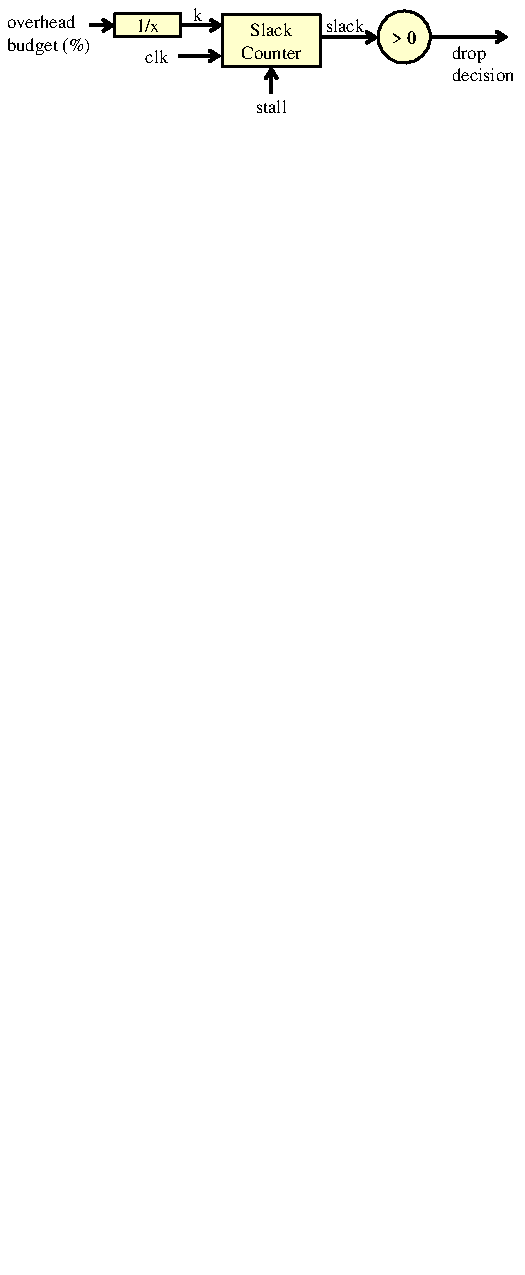
\includegraphics[width=\columnwidth]{figs/stm.pdf}
%     \vspace{-0.2in}
%     \caption{Slack tracking and drop decision hardware.}
%     \label{fig:policies.stm}
%     \vspace{-0.1in}
%   \end{center}
% \end{figure}

% Figure~\ref{fig:policies.stm} shows a hardware slack tracking module for
% keeping track of slack. 
Slack can be easily measured in hardware by using a counter that increments on every $k$-th
cycle of the main core (e.g., every 5th cycle for a 20\% target budget). 
% This $k$ can be calculated by taking the reciprocal of
% the target budget. For example, if the target budget is 20\%, then the counter
% increments on every 5th clock cycle. 
The value of this counter is the
accumulated slack. Whenever the main core is stalled due to the monitor, the
measured slack is decremented. It is difficult to precisely determine the
entire impact of monitoring on the main core due to the
difficulty in measuring certain overheads such as contention for shared memory.
However, we have found that using only the stalls due to FIFO back pressure
works well in practice.

\subsection{Deciding Which Events to Drop} 
\label{sec:policies.which}

% % Varying slack's impact on coverage for UMC
% \begin{figure}
%   \begin{center}
%     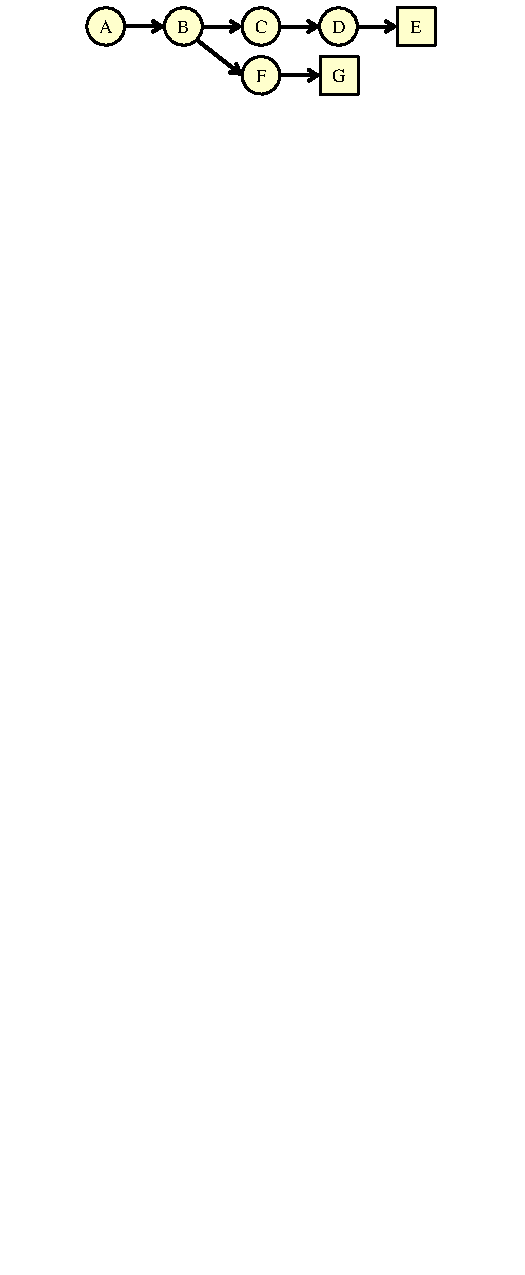
\includegraphics[width=\columnwidth]{figs/dataflow_graph.pdf}
%     \vspace{-0.3in}
%     \caption{Example dependence graph for metadata. Square nodes represent
%     events where checks are performed.} 
%     \label{fig:policies.dataflow_graph}
%     \vspace{-0.1in}
%   \end{center}
% \end{figure}

\begin{figure}
  \begin{center}
  \subfloat[unrestricted dropping]{
    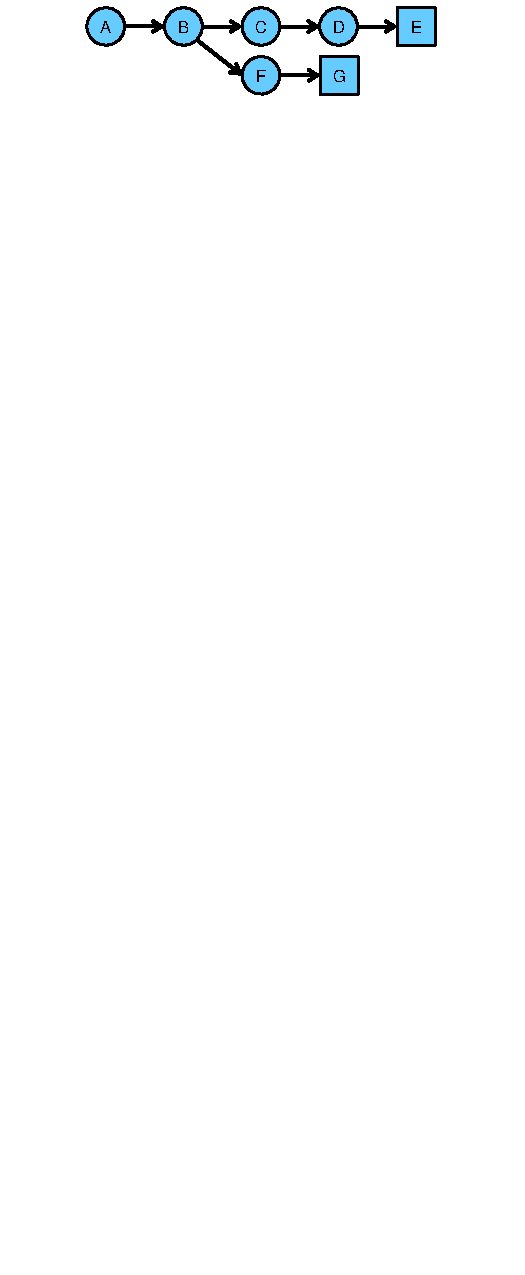
\includegraphics[width=\columnwidth]{figs/all_drop.pdf}
    \label{fig:policies.all_drop}
  }
  \vspace{-0.1in}
  \\
  \subfloat[source-only dropping]{
    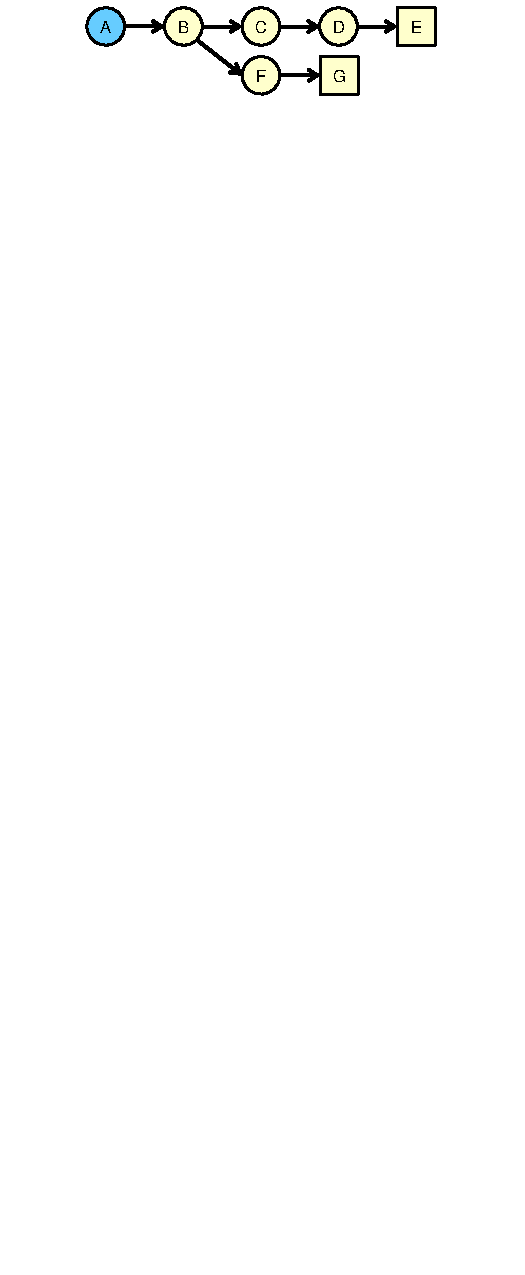
\includegraphics[width=\columnwidth]{figs/source_drop.pdf}
    \label{fig:policies.source_drop}
  }
  \vspace{-0.1in}
%   \\
%   \subfloat[sub-flow dropping]{
%     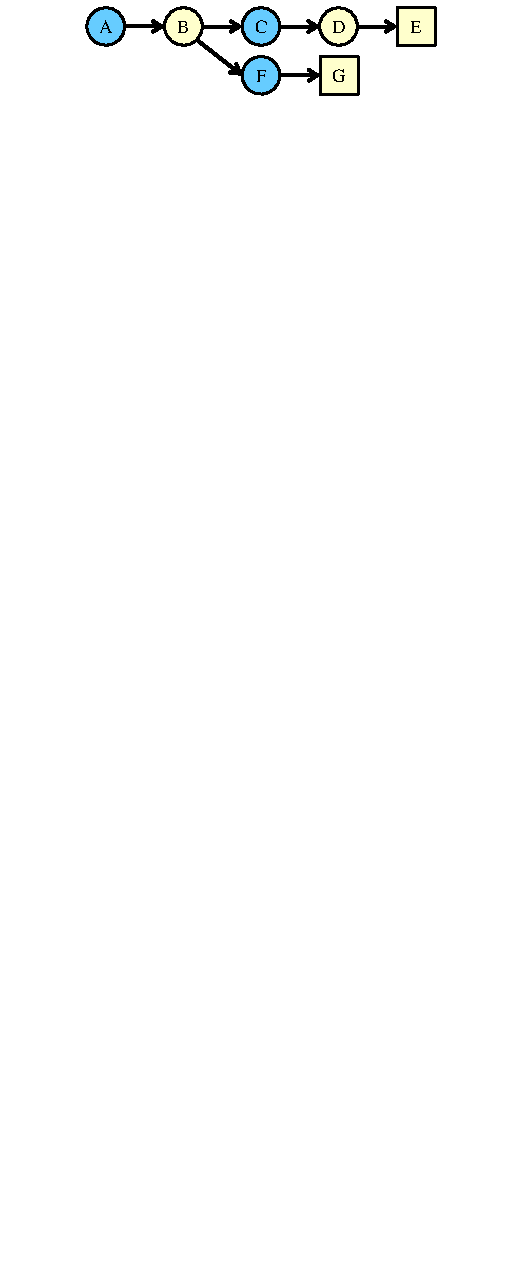
\includegraphics[width=\columnwidth]{figs/min_drop.pdf}
%     \label{fig:policies.min_drop}
%   }
  \end{center}
  \vspace{-0.1in}
  \caption{Comparison of dropping policies using metadata dependence graphs.
  Square nodes represent events where check are performed. Blue (dark) nodes
  indicate which nodes can be dropped.}
  \label{fig:policies.policies}
\end{figure}

In addition to deciding when dropping is required, trade-offs also exist in
deciding which events should be dropped.
The simplest policy is to drop any monitoring events when slack is less than or equal to zero.  However, this can result in
wasted work. For example, consider the metadata dependence graph shown in
Figure~\ref{fig:policies.all_drop}. Here, an edge from node {\tt A} to node
{\tt B} represents that if event {\tt A} is dropped, then due to its
invalidated metadata, it will cause event {\tt B} to be dropped. Square
nodes indicate events where monitoring checks are performed. In the
example, suppose that event {\tt E} is meant to perform a check operation but is dropped.
In this situation, the
monitoring operations that were done for events {\tt C} and {\tt D} were wasted
since their results were not used for any monitoring checks.
That is, by the time we decide to drop event {\tt E}, we have already 
updated metadata due to events {\tt C} and {\tt D} which is no longer needed.

An alternative dropping policy which eliminates this wasted work is to only make dropping decisions at
the root of these metadata flows. That is, we will decide to either monitor or
not monitor an entire metadata flow. We refer to this dropping decision policy
as \emph{source-only dropping} and we refer to the previous policy of 
dropping any event as \emph{unrestricted dropping}.

Figures~\ref{fig:policies.all_drop} and \ref{fig:policies.source_drop} show a
comparison of where dropping decisions are made for these two policies. Source
dropping will
result in no wasted work and thus better coverage. However, because of the coarser-grained decision, it
may be more difficult to closely match overheads. We expect source-only dropping 
to work well when there are a large number of independent metadata flows.
In addition, using a probabilistic dropping policy works poorly with
unrestricted dropping. Since each event in a dependent chain (e.g., events {\tt
A} through {\tt E}) needs to be monitored in order for the monitoring check to
be useful, randomly dropping any single event will cause the final check to be
invalid.

Depending on the target application of partial monitoring, different policies
are more applicable.
For applications where closely matching an overhead target is important, a
slack-based, unrestricted dropping policy is appropriate. However, if matching
the overhead target is not as important, then a slack-based, source-only dropping
policy could provide better coverage. 
Finally, if the goal is to use partial monitoring to enable cooperative
debugging and testing with very low overheads, then a probabilistic,
source-only dropping policy can be used to provide good total coverage over
multiple runs.

% Trade-off between source-drop and unrestricted dropping
% \begin{figure}
%   \begin{center}
%     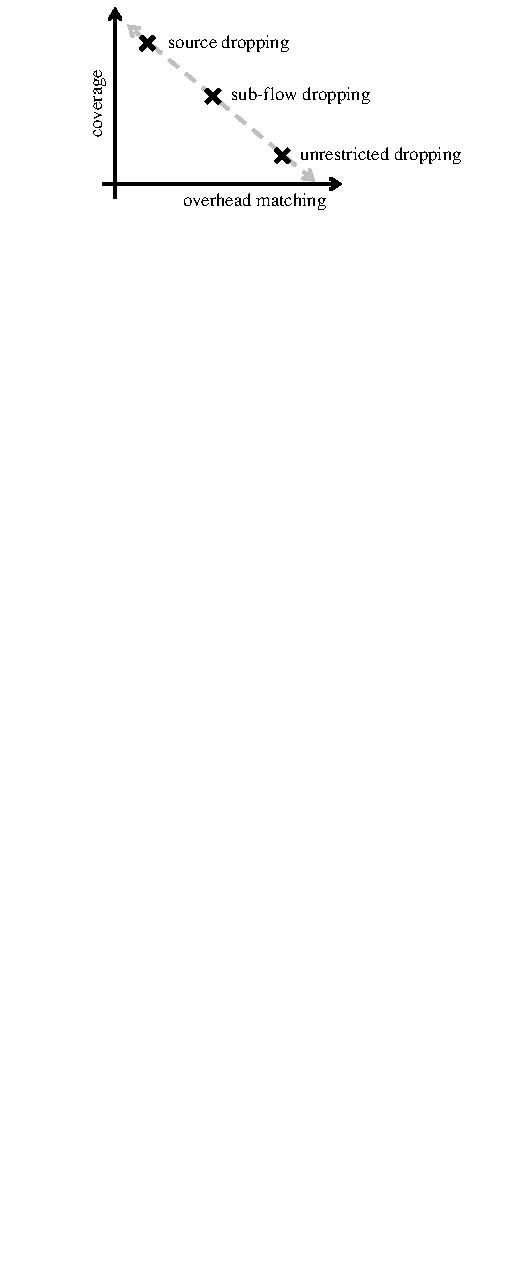
\includegraphics[width=\columnwidth]{figs/policy_trade_off.pdf}
%     \vspace{-0.3in}
%     \caption{Slack tracking and drop decision hardware.}
%     \label{fig:policies.trade_off}
%     \vspace{-0.2in}
%   \end{center}
% \end{figure}
% 
% Another possible method is to make the dropping decisions somewhere in between
% source-only dropping and unrestricted dropping. From the graph in 
% Figure~\ref{fig:policies.dataflow_graph}, we can see that if the dropping
% decision is made at event {\tt C} then we can skip event {\tt E} with no wasted
% work. If we instead choose to perform monitoring for event {\tt C}, then we want to perform all
% monitoring on that flow. Similarly, event {\tt F} creates a decision point for
% the bottom flow that will result in no wasted work and dropping event {\tt A}
% allows the entire shown metadata flow to be dropped with no wasted work. If the
% program can be
% analyzed or profiled to identify these instructions which, if dropped, lead to
% no wasted work, then this information can be used at run-time to minimize the
% amount of wasted work. We refer to this policy as \emph{sub-flow dropping}.
% Figure~\ref{fig:policies.min_drop} shows the points were dropping decisions are
% made for this policy.
% Sub-flow dropping is a coarser-grained decision than unrestricted dropping, but
% finer-grained that source-only dropping. Thus, its ability to match overheads is
% expected to sit between these other two policies. Similarly, there still exists
% edge cases where wasted work can occur, but typically we expect much less
% wasted work than unrestricted 
% dropping. Thus, we expect the coverage achieved by sub-flow dropping for a
% certain overhead to fall between source-only and unrestricted dropping. These three
% dropping policies create a trade-off space between coverage achieved and
% ability to match an overhead target.
% Figure~\ref{fig:policies.trade_off} summarizes this trade-off between coverage
% and ability to match overhead.

\section{Evaluation}
\label{sec:evaluation}

\subsection{Experimental Setup}
\label{sec:evaluation.setup}

We implemented our dataflow-guided monitoring architecture by
modifying the ARM version of the gem5 simulator \cite{gem5} to support parallel
run-time monitoring. We model the main and monitoring cores as running at 2.5
GHz with 4-way set-associative private L1 I/D caches and a shared 8-way 2 MB L2
cache. This setup is similar to the Snapdragon 801 processor commonly found in
mobile systems. The dataflow engine uses a 1 kB cache for flags.

In order to explore the generality of the architecture for
different monitors, we implemented three different monitors: uninitialized
memory check (UMC), array bounds check (BC), and dynamic information flow
tracking (DIFT).  Uninitialized memory check seeks to detect loading from
memory locations that are not initialized first.  Array bounds check, as
mentioned in Section~\ref{sec:monitoring}, is a monitoring scheme that aims to
detect buffer overflows where memory accesses go beyond the boundaries of an
array. We modify the implementation of {\tt malloc} to set base and bound
metadata information. Dynamic information flow tracking is a security
monitoring scheme
which detects when information from untrusted sources is used to affect the
program control flow (i.e., indirect control instructions). For the benchmarks we consider, we mark data read from
files as untrusted. We implemented a multi-bit DIFT scheme which marks
untrusted data with a 32-bit metadata identifier so
that if an error is detected, it is possible to have information about where
the data originated from. 

We tested our system using all C benchmarks from SPECint
CPU2006 \cite{spec2006}. Since our implementation of BC depends on the
modification of {\tt malloc} to set array bounds information, we focus on the C
SPECint benchmarks. Although we do not
show results for the C++ benchmarks, we note that the results for UMC and DIFT
for these benchmarks are similar to the other results shown. For each
benchmark, we simulated for 1 billion instructions. An initial slack of 1
million cycles, which is less than 1\% of
the total execution time, is given for a 10\% target overhead. This initial
slack is scaled proportionally for other overhead targets.

\subsection{Baseline Monitoring Overheads}
% Full monitoring overheads
\begin{figure}
  \begin{center}
    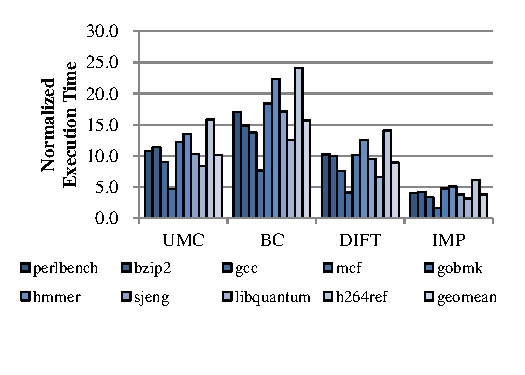
\includegraphics[width=\columnwidth]{figs/data_full_mon.pdf}
    \vspace{-0.2in}
    \caption{Full monitoring overheads for UMC, BC, and DIFT.}
    \label{fig:evaluation.full_mon}
    \vspace{-0.1in}
  \end{center}
\end{figure} Figure~\ref{fig:evaluation.full_mon} shows the execution times of
performing full monitoring normalized to the execution times of the benchmarks
without monitoring. In these results, no filtering or partial monitoring is
done. UMC shows normalized execution times from 4x to 11x with an average
of 7x. BC shows normalized execution times of 9-28x with an average of
18x while DIFT shows normalized execution times of 6x-17x with an average of
11x. One of the reasons for these high overheads is that our implementations of
these monitors dynamically allocate memory for new metadata. This can be an
expensive, many-cycle operation. Statically allocating memory for metadata
will reduce the execution time but requires a large upfront memory footprint
which caused issues with our simulator.

\subsection{Filtering of Monitoring Events}

% Full monitoring overheads
\begin{figure}
  \begin{center}
    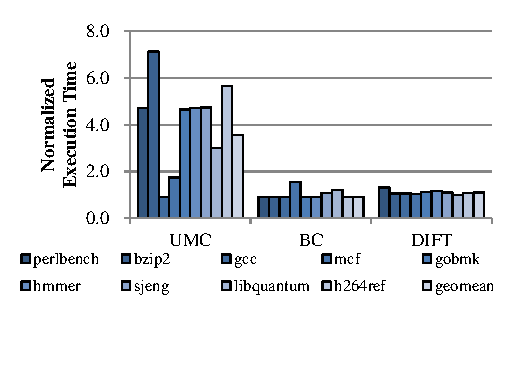
\includegraphics[width=\columnwidth]{figs/data_filtering.pdf}
    \vspace{-0.2in}
    \caption{Monitoring overheads with filtering null metadata for UMC, BC, and DIFT.}
    \label{fig:evaluation.filtering}
    \vspace{-0.1in}
  \end{center}
\end{figure}

Figure~\ref{fig:evaluation.filtering} shows the
normalized execution times with filtering enabled. We see significant
reductions in overhead for all three monitoring schemes. UMC sees normalized
execution times of 2-6x with an average of 4x with null metadata filtering. For BC, normalized execution
times drop from 18x down to 4x on average. The range of normalized execution
times for filtered BC is 1.1-17x. This is not surprising since in the baseline
implementation all loads and stores needed to be monitored. However, with
filtering, only loads and stores corresponding to arrays need to be forwarded.
Finally, DIFT sees the largest reduction in overheads with only 13\% overheads
on average after filtering, with a maximum of 42\%. This is due, in part, to the fact that
for our implementation of DIFT on SPEC
benchmarks, we only mark data read from files as tainted. For most of these
benchmarks, this propagates to relatively few instructions. Instead, if we
targeted network or streaming applications, which have larger amounts of
untrusted input data, we would expect to see less filtering.

\subsection{Coverage with Adjustable Partial Monitoring}

% BC sweep
\begin{figure*}
  \begin{center}
    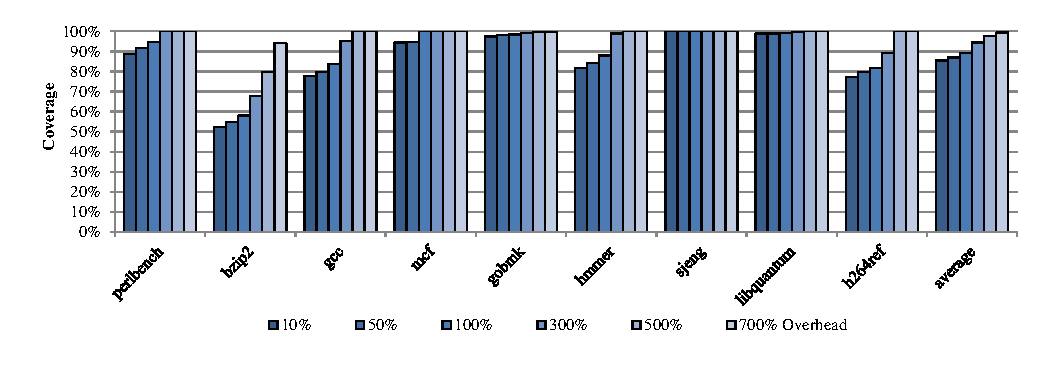
\includegraphics[width=\linewidth]{figs/data_bc_sweep.pdf}
    \vspace{-0.4in}
    \caption{Coverage versus varying overhead budget for array bounds check.}
    \label{fig:evaluation.bc_sweep}
    \vspace{-0.2in}
  \end{center}
\end{figure*}

% UMC sweep
\begin{figure*}
  \begin{center}
    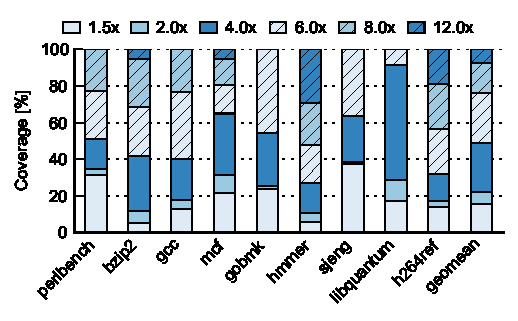
\includegraphics[width=\linewidth]{figs/data_umc_sweep.pdf}
    \vspace{-0.4in}
    \caption{Coverage versus varying overhead budget for uninitialized memory check.}
    \label{fig:evaluation.umc_sweep}
    \vspace{-0.1in}
  \end{center}
\end{figure*}

Although the overheads of DIFT are quite low after filtering, BC and UMC still
show significant overheads. In this section, we evaluate the effectiveness of
using partial monitoring (in addition to filtering) to trade-off coverage for further reduced overheads.
Figure~\ref{fig:evaluation.bc_sweep} shows the monitoring coverage achieved by
array bounds check as we vary the overhead budget. 
We define \emph{monitoring coverage} as the 
percentage of checks that are performed 
(indirect jumps in DIFT, loads in UMC, and memory accesses in BC). 
The metric is chosen to understand
how likely an error/attack instance is to be detected on an individual system. 
While we could not evaluate real errors/attacks due to difficulty in setting up
a large number of bugs and exploits, we believe that the percentage of checks
provides a good estimate of detection probability when errors/attacks are 
uniformly distributed across checks.
Note that this metric is different from the
percentage of monitoring events that are not dropped, which includes
non-check instructions.

We see that by varying the overhead budget, the coverage achieved also varies.
With only a 10\% overhead budget, array bounds check still
achieves 82\% monitoring coverage on average. The high coverage
achieved with such low overheads is due to two main effects.  The first is that
monitoring can be done in parallel, providing monitoring coverage without
introducing overheads. The second effect is that, although we aggressively
filter out monitoring events, there may still exist a large number of
monitoring events that do not lead to security or reliability checks. As a
result, dropping these events can reduce overheads without a large impact on
monitoring coverage.

Figure~\ref{fig:evaluation.umc_sweep} shows the analogous graph for UMC. Again
we see that varying overhead budgets enables partial monitoring. We see that
with a 10\% overhead budget, UMC achieves 32\% monitoring coverage on average.
By increasing this overhead budget to 50\%, UMC achieves 51\% coverage. Even
higher coverage can be achieved by allowing higher overheads.

\subsection{Comparing Dropping Policies}

% UMC exec time
\begin{figure}
  \begin{center}
    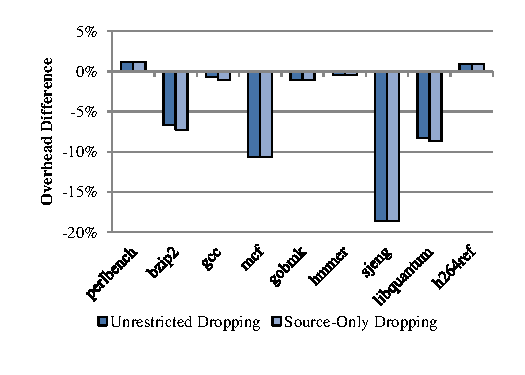
\includegraphics[width=\columnwidth]{figs/data_umc_exec_time.pdf}
    \vspace{-0.2in}
    \caption{Error in meeting overhead budget for uninitialized memory check for different dropping policies.}
    \label{fig:evaluation.umc_exec_time}
    \vspace{-0.2in}
  \end{center}
\end{figure}


% UMC coverage across policies
\begin{figure}
  \begin{center}
    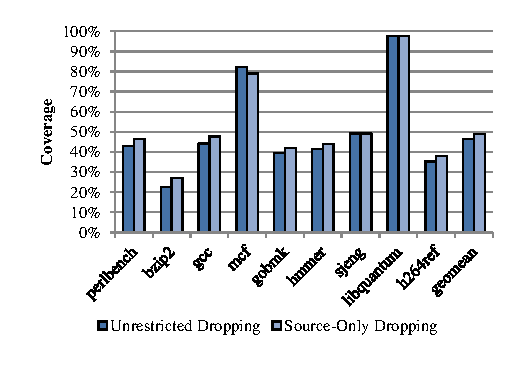
\includegraphics[width=\columnwidth]{figs/data_umc_coverage.pdf}
    \vspace{-0.2in}
    \caption{Coverage for uninitialized memory check for different dropping policies.}
    \label{fig:evaluation.umc_coverage}
    \vspace{-0.1in}
  \end{center}
\end{figure}
In this section we evaluate the trade-offs between unrestricted dropping and source-only dropping.
Figure~\ref{fig:evaluation.umc_exec_time} shows the difference between the
overhead budget and the run-time monitoring overheads for UMC. A positive value
means that the overhead target was overshot while a negative value indicates
that the overhead budget was met. We see similar results for unrestricted
dropping and source-only dropping due to the fact that UMC consists of a large
number of independent monitoring flows.
Figure~\ref{fig:evaluation.umc_coverage} shows the coverage of UMC for
unrestricted dropping and source-only dropping. We see that source-dropping
consistently achieves higher coverage than unrestricted dropping. This is due
to the fact that some of the overheads of monitoring for unrestricted dropping
are being spent on wasted work as discussed in Section~\ref{sec:policies.events}.

% BC exec time
\begin{figure}
  \begin{center}
    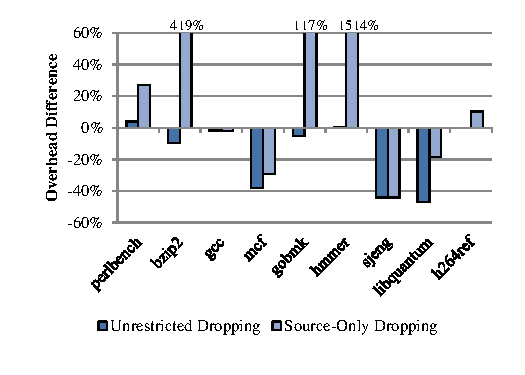
\includegraphics[width=\columnwidth]{figs/data_bc_exec_time.pdf}
    \vspace{-0.2in}
    \caption{Error in meeting overhead budget for array bounds check for different dropping policies.}
    \label{fig:evaluation.bc_exec_time}
    \vspace{-0.2in}
  \end{center}
\end{figure}

% BC coverage across policies
\begin{figure}
  \begin{center}
    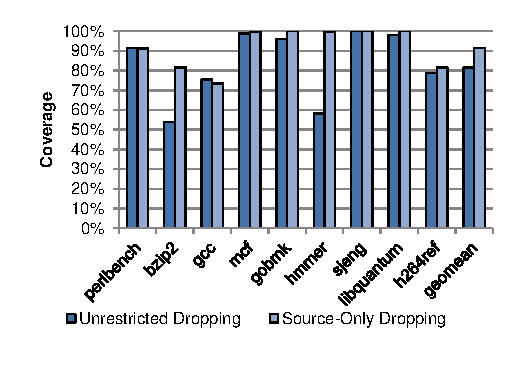
\includegraphics[width=\columnwidth]{figs/data_bc_coverage.pdf}
    \vspace{-0.2in}
    \caption{Coverage for array bounds check for different dropping policies.}
    \label{fig:evaluation.bc_coverage}
    \vspace{-0.2in}
  \end{center}
\end{figure}

Next, we evaluate these trade-offs between source-only dropping and unrestricted dropping for BC.
Figure~\ref{fig:evaluation.bc_exec_time} shows the overhead differences for BC
and Figure~\ref{fig:evaluation.bc_coverage} shows the coverage for BC.
From Figure~\ref{fig:evaluation.bc_exec_time}, we see that for several
benchmarks, source-only drop fails to meet the specified overhead target.
The overshoot of the overhead target is quite high with an overhead difference
of 420\% for {\tt bzip2}, 120\% for {\tt gcc}, and 1500\% for {\tt hmmer}.
Since only array allocations are considered source events for BC, it is
difficult for source-only dropping to match overhead targets. Although
Figure~\ref{fig:evaluation.bc_coverage} again shows higher coverage for
source-only dropping, this is in part due to the fact that is running with
higher overheads.

\subsection{Multiple-Run Coverage}

% Multi-run coverage with unrestricted dropping
\begin{figure}
  \begin{center}
    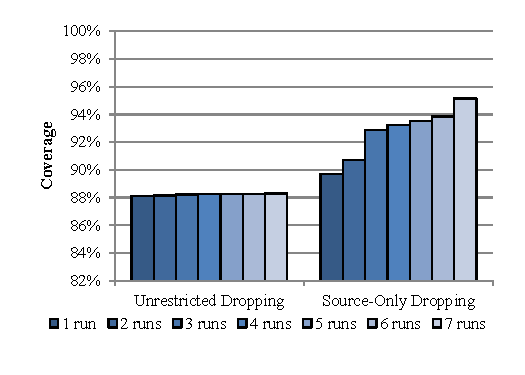
\includegraphics[width=\columnwidth]{figs/data_multirun_coverage.pdf}
    \vspace{-0.2in}
    \caption{Coverage over multiple runs for BC at 10\% overhead with an unrestricted dropping policy.}
    \label{fig:evaluation.multirun}
    \vspace{-0.1in}
  \end{center}
\end{figure}

One possible application of partial monitoring with low overheads is to enable
cooperative debugging. The idea with cooperative debugging is to use partial
monitoring with very low overheads across a large number of users or runs. By
varying the pattern of partial monitoring done on each run, the goal is to
achieve high coverage across multiple runs. Varying the monitoring that is
done for different runs can be achieved by introducing some randomness into the
dropping decision. Figure~\ref{fig:evaluation.multirun} shows the total
coverage achieved over multiple runs for array bounds check running with a 10\%
overhead budget and an unrestricted dropping policy. Each run was simulated for
100 million instructions. For these simulations, events were
dropped probabilistically with the probability scaled proportionally to slack.
That is, when slack is high, the probability of dropping is low and the
probability increases as we run out of slack. We see that the coverage achieved
quickly asymptotes for an unrestricted dropping policy. This is due to the fact
that since there are multiple dependent monitoring operations that must be done
in order for a final check to be successful, a small amount of randomness at
each event quickly compounds to reduce the probability of certain checks to
near zero. Instead, source-only dropping is much better suited for achieving high
coverage over multiple runs.

\subsection{Area and Power Overheads}

% Area and Power Overheads
\begin{table}[tb]
  \begin{center}
    \vspace{-0.0in}
    \begin{footnotesize}
    
% Full monitoring at zero slack

\begin{tabular}{|c|c|c|}
\hline

{\bf Monitor} & {\bf Peak Power [mW]} & {\bf Runtime Power [mW]} \\ \hline\hline

UMC  & 4.7 (4.9\%) &  3.1 (8.2\%) \\ \hline
BC   & 6.9 (7.1\%) &  4.1 (10.7\%) \\ \hline
DIFT & 7.2 (7.4\%) &  4.3 (11.1\%) \\ \hline

\end{tabular}

    \end{footnotesize}
    \caption{Average power overhead for dropping hardware at a 50\% overhead
    budget. Percentages in parentheses are normalized to the main core
    power.}
    \vspace{-0.2in}
    \label{tab:evaluation.area_power}
  \end{center}
\end{table}

Adding the dataflow engine in order to enable filtering and partial monitoring adds
overheads in terms of area and power. We use McPat \cite{mcpat-micro09} to get
a first-order estimate of these area and power overheads in a 40 nm technology
node. McPat estimates the main core area as 2.71 mm$^2$ and the peak power usage as
965 mW averaged across all benchmarks. The average runtime power usage was 385 
mW. These area and power numbers consist of the core and
L1 cache, but do not include L2 cache, memory controller, and other
peripherals. The power numbers include dynamic as well as static (leakage)
power. For the dataflow engine, we modeled the ALUs used for address
calculation, the dataflow flag register file and cache, the configuration
tables, and the filter decision table. These were modeled using the
corresponding memory and ALU objects in McPat. We
note that this is only a rough area and power estimate since components such as the
wires connecting these modules have not been modeled. However, this gives a
sense of the order-of-magnitude overheads involved with implementing our
approach.

Our results show that an additional 0.197 mm$^2$ of silicon area is needed, an
increase of 7\% of the main core area. Table~\ref{tab:evaluation.area_power}
shows the peak and runtime power overheads averaged across all benchmarks with
a 50\% monitoring overhead target. The peak power is 5-7 mW, which is
less than 1\% of the main core's peak power usage. Similarly, the average runtime power is 3-4 
mW, corresponding to about 1\% of the main core's runtime power.


\section{Related Work}
\label{sec:related}

% Monitoring
Many monitoring schemes have been developed for various security, reliability,
debugging, and other capabilities. There exist monitoring schemes for uninitialized
memory check \cite{mondrian-asplos02}, array bounds check
\cite{hardbound-asplos08, clause-ase07}, and dynamic information flow
tracking \cite{dift-asplos04, raksha-isca07, loki-osdi08}.
Memtracker \cite{memtracker-hpca07} uses monitoring to check for various
memory-related bugs and errors.  Control flow verification techniques perform
monitoring to check that program execution follows expected control flows
\cite{schuette-comp87, impres-dac06,
kayaalp-isca12}.  Our monitoring architecture is designed to
be generally applicable to any of these instruction-grained monitoring schemes.
% In particular, our proposed architecture may be especially useful for some of
% these more complex schemes which also have higher overheads.  Similarly,
% although many of these schemes showed low overheads in custom hardware, our
% architecture can be used to reduce the overheads when applying these schemes on
% a multi-core platform.
 
% Filtering
FADE \cite{fade-hpca14} presents a general filtering engine in order to reduce
the overheads of monitoring. It filters out redundant updates and null checks
by reading metadata values. 
By extending our dataflow engine for partial monitoring, we are able to also
filter out null checks as well as null metadata propagations, but we do not
handle filtering redundant updates.
% We are able to do this because the dataflow engine can also
% propagate the null information.  
In contrast to FADE, our dataflow engine only
requires reading and writing 2-bit flags rather than the entire metadata. 
% As
% we have shown, our dataflow engine also enables adjustable overheads without
% false positives which is not a capability described by FADE.

% Sampling
Statistical sampling is a method that has been applied to various debugging
techniques in order to reduce their performance overheads. For example, Liblit
et al. sampled program runs of thousands of users in order to find bugs
\cite{liblit-pldi05}. This idea has also been applied to detecting memory
leaks~\cite{chilimbi-asplos04}, dataflow analysis~\cite{greathouse-cgo11}, and
other run-time monitoring techniques. The Testudo project
\cite{testudo-micro08} specifically targets hardware-based run-time monitors.
These sampling-based techniques all limit the debugging capabilities in order
to provide lower performance overheads, similar to our architecture's goals.
However, these approaches are not able to explicitly set an overhead budget, as
our system is able to do. In addition, with the exception of Testudo, these
methods have not considered parallel monitoring. Our techniques for generally
reducing the overheads of monitoring can also be used to enable these
low-overhead, multi-user/run debugging techniques.

% Limited Monitoring
In terms of partial monitoring, the Quality Virtual Machine (QVM) is a
modification of the Java Virtual Machine (JVM) that supports run-time
monitoring with controllable overheads \cite{qvm-oopsla08}. Similarly, Huang et
al. created a framework for controlling the overheads of software-based
monitoring \cite{huang-sttt12}. These projects are targeting a similar problem
to the one we address in this paper. However, both projects are focused on
software-based monitoring and thus their mechanisms modify the software
monitoring framework in order to enable or disable monitoring. Instead, our
architecture provides a general hardware mechanism to control overheads of
parallel monitoring architectures. In addition, these works prevented
false positives by enabling and disabling monitoring using only a source-dropping
policy. Lo et al. \cite{lo-rtas14} developed a hardware architecture to limit
monitoring in hard real-time systems. Their architecture performs unrestricted 
dropping in order to guarantee strict deadlines. 
Our system allows either source-only dropping or unrestricted dropping to be performed.
This allows the designer or user to choose the appropriate policy depending on
the monitoring scheme which has not been previously explored.

\section{Conclusion}
\label{sec:conclusion}

Parallel run-time monitoring techniques are attractive solutions for improving
the reliability, security, and debugging capabilities of systems. In this
paper, we have presented an architecture that reduces the overheads of
monitoring through filtering and adjustable partial monitoring. This is done by
using a hardware dataflow tracking engine in order to track and filter out
monitoring for null metadata. In addition, the dataflow engine tracks invalid
metdata flows in order to enable partial monitoring without false positives.
Our experimental results show that filtering can greatly reduce the average
overheads of monitoring from 7x, 18x, and 11x for UMC, BC, and DIFT down to 4x
for UMC and BC and just 13\% for DIFT. With partial monitoring, we see that
with a 50\% overhead budget, BC can still achieve 83\% coverage and UMC can
still achieve 51\% coverage. Finally, we show that although source dropping can
achieve better coverage than unrestricted dropping when it works, it is not
able to match overhead targets as well as unrestricted dropping.


%\clearpage

\bstctlcite{bstctl:etal, bstctl:nodash, bstctl:simpurl}
\bibliographystyle{IEEEtranS}
\bibliography{paper}

\end{document}

